\documentclass[11pt]{article}
\usepackage[utf8]{inputenc} 
\usepackage{amsmath,amsthm,amsfonts,amssymb,amscd}
\usepackage{multirow,booktabs}
\usepackage[table]{xcolor}
\usepackage{fullpage}
\usepackage{lastpage}
\usepackage{enumitem}
\usepackage{fancyhdr}
\usepackage{mathrsfs}
\usepackage{wrapfig}
\usepackage{setspace}
\usepackage{calc}
\usepackage{multicol}
\usepackage{cancel}
\usepackage[margin=3cm]{geometry}
\usepackage{amsmath}

\usepackage{tikz}
\usetikzlibrary{shapes,arrows}

\newlength{\tabcont}
\setlength{\parindent}{0.0in}
\setlength{\parskip}{0.05in}
\usepackage{empheq}
\usepackage{framed}
\usepackage{xcolor}
\colorlet{shadecolor}{orange!15}
\parindent 0in
\parskip 12pt
\geometry{margin=1in, headsep=0.25in}
\theoremstyle{definition}
\newtheorem{defn}{Definition}
\newtheorem{reg}{Rule}
\newtheorem{exer}{Exercise}
\newtheorem{note}{Note}
\newtheorem{Theorem}{Theorem}[section]
\newtheorem{corollary}{Corollary}
\newtheorem{Lemma}{Lemma}
\newtheorem*{Definition}{Definition}
\newtheorem*{Example}{Example}
\usepackage{accents}
\usepackage[T1,T2A]{fontenc}
\usepackage[utf8]{inputenc}
\usepackage[english]{babel}
\newcommand*\underdot[1]{%
  \underaccent{\dot}{#1}}

\begin{document}

\section{Intro}

Goals of Course

\begin{itemize}
\item overview over moder nonlinear analyses and control concepts
\item modern methodologies to analyze nonlinear systems
\item apply a wide range of nonlinear control method
learn the mathmatic basis
\end{itemize}


Differential equations $\dot x = f(x)$

Nonlinear differential eqution $\dot x = f(t,x)$

System with input $\dot x = f(x,u)$

System with input and output 
\begin{multline} 
\dot x=f(x,u) \\ y=g(x,u) 
\end{multline}

Input-output methods


Scope 
\begin{enumerate}[label={[\arabic*]}]
  \item Khalil Nonlinear System, Prentice Hall, 2002
  \item Sepulchre Constructive Nonlinear Control, Springer-Verlag 1997 
\end{enumerate}



\section{Differential equations}

Consider differential equality
\begin{equation}\label{c1:eq}
\frac{d}{dt}x(t)=\dot x(t)=f(x(t)), \ x(0)=x_0 
\end{equation}

Where $f:D\rightarrow R^n, \ D\subset R^n$ is open, [here we should explain,
what means open set].

Solution to \ref{c1:eq} $x:I_{x_0} \rightarrow D, \ t\rightarrow x(t)$ is
differentiable

Interval existence solution

Questions:

\begin{itemize}[label=$\#$]
\item existence of solution
\item "how large" is $I_{x_0}$
\item uniquence of solution
\end{itemize}



Usaly we will add some restrictions on $f$ functions, like continuous.

\subsection{Existence of solutions}

\begin{Definition}
Function $f:D \rightarrow R^n$ is contiuous at $x' \in D$ if for
$\forall \epsilon > 0 \ \exists \delta>0$ such that for $\forall x \in D$,
$\|x-x'\|<\delta => \|f(x)-f(x')\| < \epsilon$

Function $f:D \rightarrow R^n$ is continuous on D if it's 
continuous at $\forall x' \in D$
\end{Definition}

\begin{Theorem}[Piano]
If $f:D \rightarrow R^n$ continuous, then for each $x_0 \in D$\ 
$\exists x:(-\epsilon,\epsilon) \rightarrow D, \ \epsilon > 0$
satisfying (\ref{c1:eq}).
\end{Theorem}

Further, given a compact sed $U \subset D$, then 
$\exists \alpha > 0$ s.t. $\forall x_0 \in U 
\ \exists x:(-\epsilon,\epsilon) \rightarrow D$ satisfying (\ref{c1:eq}).


\begin{Example}
Consider equation $\dot x(t) = x(t)^2, \ \ x(0)=x_0=0$. Solution 
$x(t)=-\frac{1}{t-c}, \ \ c=\frac{1}{x_0}$. In this example
solution exist in interval $(-c, c)$.
\end{Example}


But, what about the number of solutions? Which conditions we should
add to garanty uniquence of solution?


\subsection{Uniquence of solutions}

\begin{Definition}
Function $f:D \rightarrow R^n$ is locally Lipshitz (continuous???) on D
if $\forall x \in D$ there is a neighborhood $N(x) \subset D$ and
$\exists L > 0$ s.t. 
\begin{equation}\label{c1:lip}
||f(x_1)-f(x_2)|| \le L ||x_1 - x_2|| 
\end{equation}

For all $x_1,x_2 \in N$.
\end{Definition}

\begin{itemize}
\item Lipschiz on $W \in D$ if (\ref{c1:lip}) holds $\forall x_1,x_2 \in W$ 
(with same L)
\item globally Lipschitz if (\ref{c1:lip}) holds $\forall x_1, x_2 \in R^n$
(with same L)
\end{itemize}


We have
\begin{itemize}[label=$\#$]
 \item localy Lipschitz functions are continuous
 \item differenciable functions are locally Lipschitz
 \item locally Lipschitz functions are Lipschitz on each compact subset of D
 	(Khalil Ex 3.19)
\end{itemize}

\begin{Lemma}[Cromwall]
Suppose that $0 \le \phi(t) \le c + L \int^t_0 \phi(\tau) d \tau$, $c,L > 0$, $\phi$ -- 
continuous. Then $\phi(t) \le c e^{Lt}$.
\begin{proof}
$c + L\int^t_0 \phi(\tau) d \tau := \psi(t)$, $\dot \psi(t) = L\phi(t) \le L \psi (t)$.

Consider $\frac{d}{dt} \left(\psi(t) e^{-LT}\right) = e^{-Lt}
\dot \psi(t)-L \psi(t) \left(\right) \le 0$, thus $\psi(t) e^{-LT}$ is
decreased, and as a result we have $\phi(t)e^{-Lt}\le \psi(t)e^{-Lt}\le \psi(0)=c$ 

\end{proof}
\end{Lemma}

\begin{Theorem}[Picard Lindelof]
If function $f:D \rightarrow R^n$ is localy Lipschitz then for $\forall x_0 \in D$
\ $\exists ! x:(-\epsilon, \epsilon) \rightarrow D, \ \epsilon > 0$
satisfying (\ref{c1:eq}).

\begin{proof}

* existence from Piano theorem

Proof of uniqueness

Consider two solutions $x_1(.)$ and $x_2(.)$ to (\ref{c1:eq}). $\dot x_1-\dot x_2=f(x_1)-f(x_2)$,
$x_1(0)=x_2(0)$. Then we can integrate equality: 
$x_1(t)-x_2(t)=\int^t_0 f(x_1(\tau))-f(x_2(\tau)) d\tau$.  
$|x_1(t)-x_2(t)| \le \int^t_0 |f(x_1(\tau))-f(x_2(\tau))| d\tau \le 
L \int^t_0 |f(x_1(\tau))-f(x_2(\tau))| d\tau$. Now we can apply Cromwall's lemma with $c=0$
and $\phi(t)=|x_1(t)-x_2(t)|$, then $\phi(t)\le 0$, then $x_1(t)=x_2(t), \ \forall t 
\in (-\epsilon,\epsilon)$
\end{proof}
\end{Theorem}

\begin{Example}
\begin{equation*}
    \dot x = 
    \begin{cases}
      \sqrt{x}, & \mbox{if } x \ge 0 \\
      0, & \mbox{else } x<0 
    \end{cases}
\end{equation*}

\begin{equation*}
    Solutions\ x(t) =
    \begin{cases}
      \frac{1}{4}(t-c)^2, & \mbox{if } t \ge c \ge 0 \\
      0, &\mbox {else} 
    \end{cases}
\end{equation*}
\end{Example}

Global existance $\&$ uniqueness
\begin{itemize}
 \item sufficient condition: $f$ globally Lipschitz
 \item another sufficient condition: solution entirely lies in a coplex set
 \item forward completeness has equivalent Lyapunov-like characterization: system is
      forward-complete iff $\exists$ solution $V:R^n \rightarrow R \ge 0$ s.t.
      $\frac{\partial V}{\partial x} f(x) \le V(x)$, $\forall x \in R^n$
\end{itemize}


\subsection{Lyapunov stability}

If functions $\dot V(x) < 0$, $\forall x \in D\\ \{0\}$, then $x^*$ is
asymptotically stable.

\begin{Definition}
Equilibrium point $x=0$ is stable if $\forall \epsilon > 0\ \exists \delta > 0$
s.t. from $\|x_0\| < \delta$ follows $\|x(t)\| \le \epsilon, \ \forall t \ge 0$.
\end{Definition}

\begin{Definition}
Equilibrium point $x=0$ is asymptotikaly stable if it stable and exist $\delta>0$
s.t. from $\|x_0\|<\delta$ follows 
$\lim_{t\rightarrow \infty}x(t) \rightarrow 0$.
\end{Definition}


\begin{Theorem}[Lyapunov's direct method]
Let $x^*=0 \in D$ be an equilibrium point of (\ref{c1:eq}), i.e., $f(0)=0.$ Let
$f: D \rightarrow R^n$ is continious. If there exist a differetiable 
$V:D\rightarrow R$ s.t. 
\begin{enumerate}
\item $V(x^*)=0$, $V(x)>0$, $\forall x \in D\\ \{0\}$
\item $\dot V(x) = \frac{\partial V}{\partial x}f(x) \le 0$, $\forall x \in D$
\end{enumerate}

then $x^*=0$ is stable.

\begin{proof}
 Fix compact $U=\{x:V(x)\le c\}$ s.t. $U\in D$. By Piano: exist $\alpha > 0$
s.t. any solution $x$ with $x_0 \in U$ exists at least on the interval
$[0,\alpha)$.

TODO proof is not full
\end{proof}
\end{Theorem}

Lyapunovs direct method gives us:
\begin{itemize}
 \item stability
 \item convergence (if $V<0$)
 \item subset of the region of attraction (all compact $U=\{x:V(x)\le c\} \in D$)
 \item existance of solution for all times
\end{itemize}





 



\section{Zero-terminal constraint MPC}

Mathematical formulation of NMPC problem:

System dynamics: $\dot x = f(x,u), \ x(0) = x_0, \ x,u \in \mathbb{R}^n$

Constraints: $x(t) \in X, \ u \in U, \ \forall t \geq 0$

Assumptions:
\begin{itemize}
\item $f(0,0) \Rightarrow x_1=0 $- equilibrium point for $u_1 = 0$
\item $f: \mathbb{R}^n \times \mathbb{R}^m \to \mathbb{R}^n$ - twice continuously differentiable
\item $U$ is a compact set (closed and bounded)
\item $X$ is a connected and closed set
\item $(0,0) \in int(X \times U)$ 
\end{itemize}

MPC optimization problem:

At time $t$, given initial state $x(t)$
\begin{equation*}
\min_{\bar u(\cdot,t)} J(x(t),\bar u(\cdot ;t))
\end{equation*}
with $J(x(t),\bar u(\cdot;t)) = \int_{t}^{t+T}L(\bar x(\tau;t),\bar u(\tau;t))d\tau$

s.t.

\begin{equation*}
\dot{\bar x} = f(x,u), \bar x(t;t) = x(t)
\end{equation*}
\begin{equation*}
\bar u(\tau;t) \in U, \bar x(\tau;t) \in X, \  \forall \tau \in [t, t +T] 
\end{equation*}
\begin{equation*}
\bar x(t+T;t) = 0
\end{equation*}

Optimal open-loop solution: 
\begin{equation*}
\bar u^* (\cdot;t) = arg\ min_{\bar u(\cdot;t)} J(x(t), \bar u(\cdot; t))
\end{equation*}

Notation used throughout the chapter:
\begin{itemize}
\item Quantities without bar: real system trajectories
\item Quantities with bar: predicted trajectories
\item $L$-stage cost
\item $(\cdot;t)$ - predicted at time $t$
\item $T$ - prediction horizon
\item Optimal value function $J^*(x(t)) = J(x(t), \bar u^*(t))$
\end{itemize}

Real trajectories deviate from predicted one!

Assumptions:
\begin{itemize}
\item $L: \mathbb{R}^n \times \mathbb{R}^m \to \mathbb{R}$ is continuous and 
\begin{equation}
\left \{
  \begin{tabular}{c}
  $L(0,0)=0$ \\
  $L(x,u) > 0$ \\
  $\forall (x,u) \neq (0,0)$
  \end{tabular}
 \right.
\end{equation}
\item $J^*(x)$ is continuous at $x=0$
\end{itemize}

MPC algorithm:
\begin{enumerate}
\item At sampling time $t$, measure $x(t)$ and solve MPC optimization problem 
\item Apply $u_{MPC}(\tau) = \bar u^*(\tau, t) \forall t \in [t, t+\delta)$ with sampling time $\delta$
\item Set $t := t + \delta $ and go to step 1
\end{enumerate}

Feasibility: The MPC problem is feasible at time $t$ if there exists at least one $\bar u(\cdot; t)$ s.t. constraints satisfied.

\begin{Theorem}
Suppose that 
\begin{enumerate}[label=(\roman*)]
\item assumptions are satisfied 
\item and that zero-terminal constraint MPC problem is feasible at $t = 0$
\end{enumerate}
Then: 
\begin{itemize}
\item MPC problem is recursively feasible 
\item resulting closed-loop system is asymptotically stable 
\end{itemize}

Let $D \subset \mathbb{R}^n$ be the set of all points for which (ii) holds. The $D$ is a region of attraction for the closed loop.

\begin{proof}

\begin{enumerate}
\item recursive feasibility: by induction
\item 
\begin{itemize}
\item feasible at $t=0$ by assumption
\item assume: feasibility at $t$. Consider the candidate solution:
\begin{equation*}
\bar u(\tau; t+\delta) =
\left \{
  \begin{tabular}{c}
  $\bar u^*(\tau;t) \ \tau \in [t+\delta, t+ T]$ \\
  $0 \ \tau \in [t+T, t+\delta+T]$ 
  \end{tabular}
  \right.
\end{equation*}
\end{itemize}
\item asymptotic stability

Idea: use $J^*(x(t))$ as "Lyapunov function"

Consider: 
\begin{equation*}
J(x(t+\delta), \bar u(\cdot;t+\delta)) = \int_{t+\delta}^{t+\delta + T} L(\bar x(\tau;t+\delta), \bar u(\tau; t+\delta))d\tau=
\end{equation*} 
\begin{equation*}
= \int_{t+\delta}^{t+T}L(\bar x^*(\tau;t), \bar u^*(\tau;t))d\tau + \int_{t+T}^{t+\delta+T}L(0,0)d\tau (=0) = 
\end{equation*}
\begin{equation*}
= J^*(x(t)) - \int_{t}^{t+\delta} L(\bar x^*(\tau;t), \bar u^*(\tau;t))d\tau
\end{equation*}
by optimality 
\begin{equation*}
J^*(x(t+\delta)) \leq J(x(t+\delta), \bar u(\cdot;t+\delta)) \leq J^*(x(t)) - \int_{t}^{t+\delta} L(\bar x^*(\tau;t), \bar u^*(\tau;t))d \tau
\end{equation*}
by induction
\begin{equation*}
J^*(x(\infty)) (\geq 0) \leq J^*(x(0)) (finite) - \int_0^{\infty}L(x_{MPC}(\tau), u_{MPC}(\tau))d\tau
\end{equation*}
\end{enumerate}
\end{proof}
\end{Theorem}

\begin{Lemma}[Barbalat's lemma]

$\phi$ uniformly continuous $\phi: \mathbb{R} \to \mathbb{R}_{\geq 0}$
\begin{equation*}
\lim_{t \to \infty} \int_0^t \phi(\tau)d\tau < \infty \Rightarrow \phi(t)\to 0, t \to \infty
\end{equation*}
\end{Lemma}
From Barbalat's lemma
$L \to 0 $ when $t \to \infty \Rightarrow $ L pos.def. $\|x_{MPC}(t)\| \to 0$ when $t \to \infty \Rightarrow$ convergence

Lyapunov stability: using standard arguments ($J^*$ is continuous at $x=0$)

Lessons learned:
\begin{itemize}
\item feasibility $\Rightarrow$ stability
\item value function is Lyapunov function
\item have to prove recursive feasibility
\item suboptimal solution is sufficient for stability  
\end{itemize}



\section{Quasi - infinite horizon MPC}

Goal: Relax (restrictive) zero-terminal zero-terminal constraint

Idea: terminal region + local CLF(controller Lyapunov functiom)

MPC optimization problem: At time $t$
\begin{equation*}
\min_{\bar u(\cdot;t)} J(x(t),\bar u(\cdot;t)) = \int_t^{t+T}L(\bar x(\tau;t), \bar u(\tau;t))d\tau + F(\bar x(t+T;t)) 
\end{equation*}

$F(\bar x(t+T;t))$ - terminal cost

s.t.

\begin{equation*}
\dot{\bar x} = f(\bar x, \bar u), \bar x(t;t) = x(t)
\end{equation*}
\begin{equation*}
\bar x(t;t) \in X \ \bar u(t;t) \in U \ \forall \tau \in [t,t+T]
\end{equation*}
\begin{equation*}
\bar x(t+T;t) \in X^f
\end{equation*}

$X^f$ - terminal region

Optimal solution: $\bar u^*(\cdot, t), \ J^*(x(t))$

Assumption 1: Terminal region + terminal controller

There exists an auxillary local controller $u = k^{loc}(x)$ s.t.
\begin{enumerate}
\item $X^f$ is positively invariant $\dot x = f(x,k^{loc}(x))$
\item $k^{loc}(x) \in U \ \forall x \in X^f$
\item $\dot F(x) + L(x, k^{loc}(x)) \leq 0 \ \forall x \in X^f$
\end{enumerate}

$\Rightarrow$ F is a local control-Lyapunov function.

\begin{Theorem}

Suppose Assumption 1 holds and MPC problem is feasible at $t=0$. Then:
\begin{itemize}
\item recursive feasibility
\item closed-loop is asymptotically stable
\end{itemize}

\begin{proof}
\begin{enumerate}
\item Recursive feasibility by induction 
\begin{itemize}
\item feasible at $t=0$ by assumption
\item assume feasibility at $t$
\end{itemize}
candidate 
\begin{equation*}
\bar u(\tau; t+\delta) =
\left \{
  \begin{tabular}{c}
  $\bar u^*(\tau;t) \ \tau \in [t, t+ T]$ \\
  $k^{loc}(\bar x(\tau;t+\delta)) \ \tau \in [t+T, t+\delta+T]$ 
  \end{tabular}
  \right.
\end{equation*}
$\Rightarrow$ this is a feasible solution at $t+\delta$
\item asymptotic stability
\begin{equation*}
J^*(x(t+\delta)) - J^*(x(t)) \leq J(x(t+\delta), \bar u(\cdot;t+\delta)) - J^*(x(t)) =
\end{equation*}
\begin{equation*}
\int_{t+\delta}^{t+ \delta +T} L(\bar x(\tau;t+\delta), \bar u(\tau;t+\delta)) d\tau + F(\bar x(t+\delta+ T;t+\delta)) -
\end{equation*}
\begin{equation*}
- \int_{t}^{t+T}L(\bar x^*(\tau;t),\bar u^*(\tau;t))d\tau - F(\bar x^*(t+T;t)) =
\end{equation*}
\begin{equation*}
= \int_{t+T}^{t+\delta+T}L(\bar x(\tau;t+\delta), k^{loc}(\bar x(\tau;t+\delta)))d\tau + F(\bar x(t+\delta+T;t+\delta)) -
\end{equation*}
\begin{equation*}
- \int_t^{t+\delta}L(\bar x^*(\tau;t), \bar u^*(\tau;t))d\tau - F(\bar x^*(t+T;t)) \leq
\end{equation*}
As far as from Assumption 1.3 we have the sum of three terms is $\leq 0$
\begin{equation*}
-\int_t^{t+\delta}L(\bar x^*(\tau;t),\bar u^*(\tau;t))d\tau
\end{equation*}
$\Rightarrow J^*(x(\infty)) \leq J^*(x(0)) - \int_0^{\infty}L(x_{MPC}(\tau), u_{MPC}(\tau))d\tau$
From here: some steps as in zero-terminal constraint rose. 
\end{enumerate}
\end{proof}
\end{Theorem}

How can Assumption 1 be satisfied?

Assume:
\begin{itemize}
\item quadratic state cost $L(x,u) = x^TQx + u^TRu, \ Q,R >0$
\item linearization at the origin is stabilizable 
$\dot x = Ax+Bu \ A = \frac{\partial F}{\partial x}(0,0) \ B = \frac{\partial F}{\partial u}(0,0)$
\end{itemize} 

Approach: 
\begin{itemize}
\item Linear auxiliary controller $k^{loc}(x)=Kx$
\item Quadratic terminal cost function $F(x) = x^TPx$, $P > 0$
\item Terminal region $X_{\alpha}^f = \{x \in \mathbb{R}^n | x^TPx \leq \alpha\}$ for some $\alpha > 0$
\item Determine $P,K,\alpha$ s.t. Assumption 1.1-1.3 hold:
\end{itemize}
For (Assumption 1.3):
\begin{equation*}
\frac{d}{dt}x(t)^TPx(t) \leq - x(t)^t(Q + K^TRK)x(t) = - x(t)^TQ^*x(t)
\end{equation*}
[$x^TQx + u^TRu = [u=Kx] = x^T(Q+K^TRK)x)$]
\begin{equation*}
\frac{d}{dt}x(t)^TPx(t) = f(x,Kx)^TPx + x^TPf(x,Kx)
\end{equation*}
[$f(x,Kx) = (A+BK)x+\phi(x), A+BK = A_K$, $K$ is chosen s.t. $A_BK$ is Hurwitz]

Upper bound for $x^TP\phi(x)$:
$L_{\phi} := sup\{ \frac{|\phi(x)|}{|x|}, x \in X_{\alpha}^{f}, x \neq 0\}$
\begin{equation}\label{nonlinearity_inequality}
x^TP\phi(x) \leq |x^TP| |\phi(x)| \leq \| P\| L_{\phi} |x|^2 \leq \frac{\|P\|L_{\phi}}{\lambda_{min}(P)}x^TPx
\end{equation}

We choose $\alpha$ small enough s.t. 
\begin{equation}\label{alpha_choice}
L_{\phi} \leq \frac{k \lambda_{min}(P)}{\|P\|} 
\end{equation}
for some $k > 0$. Plug this into (\ref{nonlinearity_inequality}): $x^TP\phi(x) \leq kx^TPx$. 
Insert this into $\frac{d}{dt}x^TPx \leq x^T(A_KP + PA_K)x + 2kx^TPx$
\begin{equation*}
= x^T((A_K + kI)^TP + P(A_K+kI))x
\end{equation*}
ensure that it $\leq - x^TQ^*x$

$\Rightarrow$ Lyapunov equation which can be solved if any only if $A_K + kI$ is Hurwitz 
\begin{equation}\label{k_choice_inequality}
\Leftrightarrow k < - max\ Re \{ \lambda(A_K)\}
\end{equation}

\begin{equation}\label{lyapunov_equation}
\Rightarrow\ (A_K + kI)^TP + P(A_K + kI) = - Q^*
\end{equation}

Design procedure 
\begin{enumerate}
\item Compute $K$ s.t. $(A+BK)$ is Hurwitz 
\item Choose $k > 0$ s.t. (\ref{k_choice_inequality}) and solve (\ref{lyapunov_equation})
\item Find largest possible $\alpha_1$ s.t. $Kx \in U, \ \forall x \in X^f_{\alpha}$ 
\item Find the largest $\alpha \in (0,\alpha_1]$ s.t. (\ref{alpha_choice}) holds
\end{enumerate}

Alternative to the (4) step

Solve optimization problem 
\begin{equation}
\max_{x} x^TP\phi(x) - kx^TPx s.t. \ x^TPx \leq \alpha
\end{equation}

Iterate this by reducing $\alpha$ from $\alpha_1$ until optimal value of (4) is nonpositive

Degrees of freedom in design
\begin{itemize}
\item calculation of $K$
\item choice of $k$ - tradeoff between "large" terminal region and "large" $P$
\end{itemize}


\section{Unconstrained MPC}\label{chap3}

Goal:Guarantee stability + degree of suboptimality
without stabilizing terminal constraint + cost

Setup: 
\begin{itemize}
\item $\dot x = f(x,u), x(0)=x_0$
\item input constraints $u(t) \in \mathbb{U} \subseteq \mathbb{R}^m \forall t \geq 0$
\end{itemize}

Infinite-horizon cost function:
$J_{\infty}(x_0, \bar{u}(\cdot; 0)) = \int_{0}^{\infty}L(\bar x(\tau;0), \bar u(\tau;0))d\tau  \Rightarrow$ optimal value function $J_{\infty}^*(x_0)$

Assumption: $J^{*}_{\infty}(x_0) < \infty, \forall x_0 \Rightarrow$ system is asymptotically stabilizable

Finite-horizon cost function:
$J_{T}(x(t), \bar{u}(\cdot; t)) = \int_{0}^{T}L(\bar x(\tau;t), \bar u(\tau;t))d\tau$

Infinite-horizon performance resulting from application of MPC controller:

$J_{\infty}^{MPC}(x_0) = \int_{0}^{\infty}L(\bar x_{MPC}(\tau), \bar u_{MPC}(\tau))d\tau$

\begin{Definition}
Suboptimality index $\alpha$:
$\alpha J_{\infty}^{MPC}(x_0) \leq J_{\infty}^{*}(x_0) \forall x_0$

\begin{itemize}
\item $\alpha \leq 1$ by optimality of $J^{*}_{\infty}$
\item $\alpha > 0$ implies closed-loop stability (Barb.lemma)
\end{itemize}
\end{Definition}

Proposition 1: Relaxed dynamic programming
 
Assume $\exists \alpha \in (0,1] s.t. \forall x \in \mathbb{R}^n$

$J_{T}^{*}(x(t+\delta)) \leq J_T^*(x(t)) - \alpha\int_{t}^{t+\delta}L(\bar x^*(\tau;t),\bar u^*(\tau;t))d\tau \ \ \ (*)$

Then the estimate 
\begin{equation}\label{main_inequility}
\alpha J_{\infty}^*(x(t)) \leq \alpha J_{\infty}^{MPC}(x(t)) \leq J_T^*(x(t)) \leq J_{\infty}^*(x(t))
\end{equation}

holds for all $x \in \mathbb{R}^n$

\begin{proof}
\begin{itemize}
\item 1 and 3 inequalities follow from optimality (by definition)
\item 2 inequality follows from summing up (*) over all sampling instances
\begin{equation}
J^*_T(x(N\delta)) \leq J_T^*(x_0) - \alpha \int_0^{N\delta}L(\bar x_{MPC}(t), \bar u_{MPC}(t))dt
\end{equation}
\begin{equation}
N \to \infty : J_T^*(x_0) \geq \alpha J_{\infty}^{MPC}(x_0) 
\end{equation}
\end{itemize}
\end{proof}

Central idea (image to be inserted)

$L^*(t;t) = L(\bar x^*(\tau;t), \bar u^*(\tau;t))$

\begin{equation}\label{c_b_inequality}
(c): J_T^*(x(t+\delta)) \leq \frac{1}{\epsilon} \int_{t+\delta}^{t+T}L^*(\tau;t)d\tau :(b)
\end{equation}
\begin{equation}\label{b_a_inequality}
(b): \int_{t+\delta}^{t+T}L^*(\tau;t)d\tau \leq \gamma \int_{t}^{t+\delta}L^*(\tau;t)d\tau :(a)
\end{equation} 

\begin{Theorem}

Assume $\exists \epsilon \in (0;1]$ and $\gamma > 0$ s.t. \ref{c_b_inequality} - \ref{b_a_inequality} holds. Then (*) holds with $\alpha =1 - \gamma \frac{1-\epsilon}{\epsilon}$

\begin{proof}
\begin{equation*}
J_T^*(x(t+\delta)) - J_T^*(x(t)) = J_T^*(x(t+\delta)) - \int_{t}^{t+T}L^*(\tau;t)d\tau \leq^{(\ref{c_b_inequality})}
\end{equation*}
\begin{equation*}
\leq \frac{1-\epsilon}{\epsilon} \int_{t+\delta}^{t+T}L^*(\tau;t)d\tau - \int_t^{t+\delta}L^*(\tau;t)d\tau \leq^{(\ref{b_a_inequality})}
\end{equation*}
\begin{equation*}
\leq (\gamma \frac{1-\epsilon}{\epsilon} - 1) \int_t^{t+\delta}L^*(\tau;t)d\tau
\end{equation*} 
$-\alpha := \gamma \frac{1-\epsilon}{\epsilon} - 1$ 
\end{proof}
\end{Theorem}

Assumption 1: Asymptotic Controlability

For all x, $\exists$ some input trajectory $\hat u_x(\cdot)$
with $\hat u_x(t) \in \mathbb{U}, \forall t \geq 0$ s.t.
\begin{equation*}
L(\hat x(t),\hat u(t)) \leq \beta(t) \min_u L(x,u), \forall t > 0
\end{equation*}
with $\beta: \mathbb{R} \to \mathbb{R}_{\geq 0}$
 - continuous, positive, strictly decreasing with $\lim_{t \to 0} \beta(t) = 0$ $\Rightarrow$
$\int_0^{\infty}\beta(\tau)d\tau < \infty$
$B(t) = \int_0^t\beta(\tau)d\tau$

Typical example: (image to be inserted)

How to compute $\epsilon$ and $\gamma$:
\begin{Lemma} 
Let Assumption 1 hold. Then the inequality 
\begin{equation}\label{lemma_1_inequality}
J_T^*(x(t+\delta)) \leq \int_{t+\delta}^{t+t'}L^*(\tau;t)d\tau + B(T+\delta - t')L^*(t+t';t)
\end{equation}
holds for all $t' \in [\delta,T]$

(image to be inserted)


\begin{proof}

Consider 
\begin{equation*}
\bar u(\tau;t+\delta) = \left \{
  \begin{tabular}{c}
  $\bar u^*(\tau;t), \tau \in [t+\delta, t+t']$ \\
  $\hat u_{x'}(\tau - t - t'), \tau \in [t+t', t+\delta + T]$
  \end{tabular}
\right.
\end{equation*}
\begin{equation*}
J^*_T(x(t+\delta)) \leq J_T(x(t+\delta), \bar u(\cdot;t+\delta)) =
\end{equation*}
\begin{equation*}
=\int^{t+t'}_{t+\delta}L^*(\delta;t)d\delta + \int_{t+t'}^{t+\delta+T}L(\hat x(\tau - t - t'), \hat u (\tau - t - t'))d\tau \leq
\end{equation*} 
by Assumption 1
\begin{equation*}
\int_{t+t'}^{t+\delta+T}L(\hat x(\tau - t - t'), \hat u (\tau - t - t'))d\tau \leq L^*(t+t';t) \int_0^{T+\delta-t'}\beta(\tau)d\tau
\end{equation*}
as far as $B(t) = \int_0^t\beta(\tau)d\tau$
\begin{equation*}
\leq \int_{t+\delta}^{t+t'}L^*(\tau;t)d\tau + B(T+\delta-t')L^*(t+t';t)
\end{equation*}
\end{proof}
\end{Lemma}

Calculation of $\epsilon$ from (\ref{lemma_1_inequality}):
\begin{equation*}
J^*_T(x(t+\delta)) \leq \min_{t' \in [\delta,T]}(\int_{t+\delta}^{t+t'}L^*(\tau;t)d\tau + B(T+\delta-t')L^*(t+t';t)) \leq
\end{equation*}
\begin{equation*}
\int_{t+\delta}^{t+T}L^*(\tau;t)d\tau + B(T) \min_{t'\in[\delta,T]}L^*(t+t';t)
\end{equation*}
as far as 
$\min_{t'\in[\delta,T]}L^*(t+t';t) \leq \frac{1}{T-\delta}\int_{t+\delta}^{t+T}L^*(\tau;t)d\tau$
minimum is less or equal that the average
\begin{equation*}
=(1+\frac{B(T)}{T-\delta})\int_{t+\delta}^{t+T}L^*(\tau;t)d\tau
\end{equation*}
$(1+\frac{B(T)}{T-\delta}) = \frac{1}{\epsilon}$

\begin{Lemma}

\begin{equation*}
\int_{t+t'}^{t+T}L^*(\tau;t)d\tau \leq B(T-t')L^*(t+t';t) \forall t' \in [0;T]
\end{equation*}

\begin{proof}
Analogues to lemma 2.

Calculation of $\gamma$:

\begin{equation*}
\int_{t+\delta}^{t+T} L^*(\tau;t)d\tau \leq \int_{t+\hat t}^{t+T}L^*(\tau;t)d\tau (\forall \hat t \in [0,\delta]) \leq
\end{equation*}
\begin{equation*}
\leq \min_{\hat t \in [0, \delta]}(B(T-\hat t)L^*(t+\hat t;t)) \leq
\end{equation*}
\begin{equation*}
\leq B(T)\min_{\hat t \in [0,\delta]}L^*(t+\hat t;t) \leq \frac{B(T)}{\delta}\int_{t}^{t+\delta}L^*(\tau;t)d\tau
\end{equation*}
\end{proof}
\end{Lemma}

Denote $\gamma = \frac{B(T)}{\delta}$

$\alpha = 1 - \gamma \frac{1-\epsilon}{\epsilon} = 1 - \frac{B(T)}{\delta}(\frac{B(T)}{T-\delta})$

Alternative computation of $\epsilon$ (less conservative):

We want to compute $\epsilon$ s.t.
\begin{equation*}
\epsilon \leq \frac{\int_{t+\delta}^{t+T}L^*(\tau;t)d\tau}{J_T^*(x(t+\delta))}
\end{equation*}

Idea: Minimize 
\begin{equation}\label{minimizer_eps}
\epsilon = \min_{L_t,J^*_T}\frac{\int_{\delta}^{T}L_t(\tau;t)d\tau}{J_T^*(x(t+\delta))}
\end{equation}
$J^*_T = 1$ - without loss of generality
s.t. $0 \leq L_t \forall \tau \in [\delta,T]$
\begin{equation*}
J^*_T(x(t+\delta)) \leq \int_{\delta}^{t'}L_t(\tau)d\tau + B(T+\delta-t')L_t(t') \forall t' \in [\delta, T]
\end{equation*}
Due to linearity in $L_t$, without loss of generality we can set $J_T^* = 1$.

$\Rightarrow$ infinite dimensional linear problem

Idea for solution:
second constraint has to be active for all times 

Differentiate (\ref{lemma_1_inequality}) with relation to $t'$ 
\begin{equation*}
0 = L_t(t') + \frac{dB(T+\delta-t')}{dt'}L_t(t') + B(\tau + \delta - t') \dot L_t(t')
\end{equation*} 
as far as $\frac{dB(T+\delta-t')}{dt'} = \beta(T+\delta - t')$

\begin{equation*}
\left \{
  \begin{tabular}{c}
  $\dot L_t(t') = \frac{\beta(T+\delta - t') -1}{B(T+\delta - t')}L_t(t')$ \\
 initial condition $L_t(t)=\frac{1}{B(t)}$
  \end{tabular}
\right .
\end{equation*}

Solution:
\begin{equation*}
\bar L_t(t') = \frac{1}{B(T+\delta-t')}e^{-\int_{\delta}^{t'}\frac{1}{\beta (T+\delta-\tau)}d\tau}
\end{equation*}
Have to show: $\bar L_t$ is a minimizer of (\ref{minimizer_eps})
\begin{equation*}
\int_{\delta}^{T} \bar L_t(\tau)d\tau \leq \int_{\delta}^{T} L_t(\tau)d\tau 
\end{equation*}
for all feasible $L_t$

\begin{proof}

Assume $\exists L_t$ s.t. 
\begin{equation*}
\int_{\delta}^{T}L_t(\tau)d\tau < \int_{\delta}^{T}\bar L_t(\tau)d\tau
\end{equation*}
Then $\exists \hat t \in [\delta, T]$ s.t. $\int_{\delta}^{\hat t}L_t(\tau)d\tau \leq \int_{\delta}^{\hat t}\bar L_t(\tau)d\tau$ and $\bar L_t(\hat t) > L_t(\hat t)$

But then 
\begin{equation}
1 = \int_{\delta}^{\hat t} \bar L_t(\tau)d\tau + B(T+\delta-\hat t)\bar L_t(\hat t) > \int_{\delta}^{\hat t}L_t(\tau)d\tau + B(T+\delta-\hat t) L_t(\hat t)
\end{equation}

the sign equality from (\ref{minimizer_eps}) with equality.

Contradiction:

$L_t$ cannot be a feasible solution of (\ref{minimizer_eps}) 
$\Rightarrow$ 
\begin{equation*}
\epsilon = \int_{\delta}^{T}\bar L_t(\tau)d\tau = 1 - e^{-\int_0^{T-\delta}\frac{1}{B(T-\tau)}d\tau}
\end{equation*}
\end{proof}
Similarly, better estimate for $\gamma$ can be obtained

$\alpha = 1 - \gamma\frac{1-\epsilon}{\epsilon}$
For $T \to \infty$ : both estimates for $\epsilon \to 1 \Rightarrow \alpha \to 1$ as $T \to \infty \Rightarrow$ closed-loop stability for $T$ large enough 


\section{Systems with inputs and outputs}

Study/control systems $\dot{x} = f(x,u)$ with "output" $y(t)=W(x(t))$

\subsection{Sliding mode control}

Motivating example
\begin{equation*}
\dot{x_1} = x_2
\end{equation*}
\begin{equation*}
\dot{x_2} = u \Rightarrow \dot{y} = x_2 + u
\end{equation*}
\begin{equation*}
y = x_1 + x_2
\end{equation*}

Choose:
\begin{equation*}
u =  \left\{
                \begin{array}{ll}
                  -x_2-1, \ \ y > 0\\
                  -x_2+1, \ \ y < 0\\
                  -x_2, \ \ y=0
                \end{array}
              \right. 
\end{equation*}
\begin{equation*}
\Rightarrow \dot y =  \left\{
                \begin{array}{ll}
                  -1, \ \ y > 0\\
                  +1, \ \ y < 0\\
                  0, \ \ y=0
                \end{array}
              \right. 
\end{equation*}

Solutions(Laratheodory) are if $y(0) > 0$, then 
\begin{equation*}
y(t) = \left\{ \begin{array}{ll}
                  y(0) - t, \ \ t \leq y(0)\\
                  0, \ \ t > y(0)
                \end{array}
              \right. 
\end{equation*}
If $y(0) < 0$, then
\begin{equation*}
y(t) = \left\{ \begin{array}{ll}
                  y(0) + t, \ \ t \leq y(0)\\
                  0, \ \ t > -y(0)
                \end{array}
              \right. 
\end{equation*}

%TODO picture

Key property: choose $u$ s.t. $y(t)$ goes to zero in finite time $\Rightarrow x(t)$ tends $\{ (x_1, x_2) \in \mathbb{R}^2 | x_1 +x_2 = 0 \}$ in finite time

Consider dynamics on $S$
\begin{equation*}
\left\{ \begin{array}{l}
                  \dot{x_1} = x_2 (x_2 = -x_1 \ $if$ \  y =1) = -x_1\\
                 \dot{x_2} = u = -x_2
                \end{array}
              \right. 
\end{equation*} 
globally as stable

%TODO picture

Two "phases"
\begin{enumerate}
\item solutions converge to $S$ in finite time
\item solutions converge to zero ("on S") asymptotically
\end{enumerate}
$\leadsto $ "sliding mode" control

Remark: in (1) "finite time convergence is crucial"

General procedure:
\begin{equation*}
\dot{x} = f(x)+g(x)u \\
y = h(x)= s(x)
\end{equation*}
$f: \mathbb{R}^n \to \mathbb{R}^n, \  y : \mathbb{R}^n \to \mathbb{R}^n, \ s: \mathbb{R}^n \to \mathbb{R}$

$u$ - scalar input, $s(x)$ - sliding

single input, single output 

Assumptions: $y$ has relative degree 1, well - defined globally, i.e. $L_gs(x) \neq 0 \ \forall \in \mathbb{R}^n$



\section{Input/Output Methods}

References: Desoev, Vidyasagar "Feedback Systes Input-output properties"

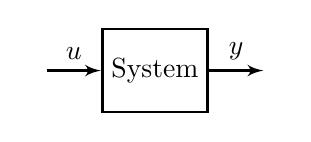
\begin{tikzpicture}[auto,>=latex']
    \tikzstyle{block} = [draw, shape=rectangle, minimum height=3em, minimum width=3em, node distance=2cm, line width=1pt]
    \tikzstyle{sum} = [draw, shape=circle, node distance=1.5cm, line width=1pt, minimum width=1.25em]
    \tikzstyle{branch}=[fill,shape=circle,minimum size=4pt,inner sep=0pt]
    \tikzstyle{tmp} = [coordinate]
    %Creating Blocks and Connection Nodes
    \node at (-1.5,0) (input) {};
    \node [block] (sys) {System};
    \node at (1.5,0) (output) {};
    %Conecting Blocks
    \begin{scope}[line width=1pt]
         \draw[->] (input) -- node{$u$} (sys);
         \draw[->] (sys) -- node{$y$} (output);
    \end{scope}
\end{tikzpicture}

\begin{equation*}
\begin{split}
&u: u\rightarrow y \\
&u,y:[0,\infty]\rightarrow \mathbb{R}^m \\
&t \rightarrow u(t), y(t)
\end{split}
\end{equation*}

\subsection{Sygnals and Systems}

\begin{itemize}
\item How to define "stability" in input/output setting?
\item Which signals are "good"?
\end{itemize}

\begin{Definition}
 $Lp$-spaces, $p\in[1,\infty]$. 
 $Lp[0,\infty) = \{\Phi:[0,\infty)\rightarrow\mathbb{R}^m, measurable|
  \int_0^\infty ||\Phi(t)||^p dt < \infty\}$
\end{Definition}

Interpretation: "finite energy sygnal" (p=2).

Remark: "measurable" = pointwise limit of a sequence of piecewise constant functions
(except on a set of measure 0)

\begin{Example}:

\begin{itemize}
 \item[-] continuous function
 \item[-] functions with "few enough" discontinuities
\end{itemize}
\end{Example}

$Lp$ is a real vector space ("signals $\Phi(\cdot)$ are vectors") i.e., for 
$\Phi, \Phi_1, \Phi_2 \in Lp$, $\alpha \in \mathbb{R}$ vector addition:
$\Phi_1+\Phi_2:t \rightarrow \Phi_1(t)+\Phi_2(t) \in Lp$. Scalar multiplication:
$\alpha \Phi:t\rightarrow \alpha\Phi(t) \in Lp$

Zero element is signal $\Phi \equiv 0$.

$Lp$ is a normed vector space with norm $||\Phi||_{Lp}=\sqrt[p]{\int_0^\infty ||\Phi(t)||^p dt}$
for $\Phi \in Lp$ $\Rightarrow$
\begin{itemize}
 \item $||\Phi||_{Lp}=0 \iff \Phi=0$, else $||\Phi||_{Lp}>0$
 \item for $\alpha \in \mathbb{R}$, $||\alpha\Phi||_{Lp}=|\alpha| ||\Phi||_{Lp}$
 \item for $\Phi_1, \Phi_2 \in Lp\ $ $||\Phi_1+\Phi_2||_{Lp} \le ||\Phi_1||_{Lp}+||\Phi_2||_{Lp}$
\end{itemize}

For $p \to \infty$ set of all measurable and (essentially) bounded functions $L_{\infty}$, for continuous $\phi$ 
\begin{equation*}
\|\phi\|_{L_{\infty}} = \inf \{ c \in \mathbb{R} | \|\phi(t)\| \leq c\ a.e.\} = \sup_{t > 0} \| \phi(t)\|
\end{equation*}
%TODO picture

\begin{Example}
\begin{equation*}
\phi (t) = e^{- \alpha t}, \ \alpha > 0, \ p \in [1,\infty )
\end{equation*}
\begin{equation*}
\begin{split}
\|\phi \|_{L_p} = \sqrt[p]{\int_0^{\infty} \|e^{-\alpha t}\|^p dt} = \\
= \sqrt[p]{[-\frac{1}{\alpha p}e^{-\alpha pt}]_0^{\infty}} = \sqrt[p]{\frac{1}{\alpha p}} < \infty \\
\Rightarrow \phi \in L_p \ \forall p \in [1, \infty) \ p= \infty : \\
\sup_{t \geq 0} \phi (t) = \phi (0) = 1 \Rightarrow p \in L_{\infty}
\end{split}
\end{equation*}
\end{Example}

Special case $p = 2$ 

$L_2$ can be equipped with an inner product $\phi_1, \phi_2 \in L_2$, we write $<\phi_1, \phi_2>_{L_2} :=  \int_0^{\infty} \phi_1(t)^T\phi_2(t)dt$

symmetry $<\phi_1, \phi_2>_{L_2} = <\phi_2, \phi_1>_{L_2}$

(bi- )linearity 
\begin{equation*}
\begin{split}
<\alpha \phi_1, \phi_2>_{L_2} = \alpha <\phi_1, \phi_2>_{L_2} \ \alpha \in \mathbb{R} \\ 
<\phi_1 + \phi_2, \phi_3>_{L_2} = <\phi_1, \phi_3>_{L_2} + <\phi_2, \phi_3>_{L_2}, \ \phi_3 \in L_2 
\end{split}
\end{equation*}

positive definiteness: $<\phi_1, \phi_1>_{L_2} = 0$ iff $\phi_1 = 0$, $<\phi_1, \phi_1>_{L_2} > 0$ else.

$\Rightarrow (L_2, <\cdot, \cdot>_{L_2})$ is an inner product space

$\|\ \phi|_{L_2}^2 = < \phi, \phi>_{L_2}$ "induced norm". 

Particularly useful(Cauchy -Schwarz inequality) $|<\phi_1,\phi_2>_{L_2}| \leq \|\phi_1\|_{L_2}\|\phi_2\|_{L_2}$

Original motivation 

%TODO picture

\begin{Example}
\begin{equation*}
\dot{x} = x+u, \ y = x, \ x(0) = 0
\end{equation*}
$y(t) = \int_0^te^{(t-\tau)}u(t)d\tau$

Take $u(t) = \left\{
                \begin{array}{ll}
                  1, \ \ 0 \leq t \leq 1\\
                  0, \ \ t > 1
                \end{array}
              \right. $
              
Clearly, $u \in L_p$ for any $p \in [1,\infty)$. Let $t \geq 1$: 
\begin{equation*}
\begin{split}
y(t) = \int_0^1 e^{(t-\tau)}d\tau = e^t\int_0^1e^{-\tau}d\tau \\
= e^t[-e^{-\tau}]^1_0 = e^t(1-e^{-1})
\end{split}
\end{equation*}
$\Rightarrow y \not\in L_p, \ p \in [1,\infty) $.$\Rightarrow $ even that $ u \in L_p$, the output neednot be an $L_p$ - signal.
\end{Example}

Taking $H: L_p \to L_p$ does (in general) not make sense? (would be excluded too many "relevant" systems)

Meaningful longer class: extended $L_p$ spaces

Introduce "truncation operator"
\begin{equation*}
\phi_T(t) = \left\{
                \begin{array}{ll}
                  \phi (t), \ \ 0 \leq t \leq T\\
                  0, \ \ t > T
                \end{array}
              \right. 
\end{equation*}

The extension $L^e_p$ of $L_p$ is defined as 
\begin{equation*}
L^e_p = \{ \phi: [0,\infty) \to \mathbb{R}^n | \forall T \geq 0 \ \phi_T \in L_p\}
\end{equation*}
%TODO picture

$L^e_p \setminus L_p$ are "unstable" signals

\begin{Example}
$\phi (t) = e^t $ ("unstable linear system")
\begin{equation*}
\begin{split}
\|\phi_T\|^p_{L_p} = \int_0^{\infty} |\phi_T(t)|^pdt = \int_0^T|\phi(t)|^pdt =  \\
= \int_0^Te^{pt}dt = \frac{1}{p}(e^{Tp} - 1) < \infty, \ \forall T \geq 0 \\
\Rightarrow \phi \in L_p^e 
\end{split}
\end{equation*}
\end{Example}

We consider systems 
\begin{equation*}
H: u \mapsto y, L_p^e \mapsto L_p^e
\end{equation*}
and define input-output stability as follows:
\begin{Definition}
$H$ is $L_p$-stable if there exists $\alpha \in K, \ \beta \geq 0$ s.t. 
\begin{equation*}
\|(H(u))_T\|_{L_p} \leq \alpha (\|u_T\|_{L_p}) + \beta
\end{equation*}
for all $u \in L^e_p$ and all $T \geq 0$. 

$H$ is finite-gain $L_p$ stable if there exist $\gamma, \ \beta \geq 0$ s.t. 
\begin{equation}\label{finite_gain}
\|(H(u))_T\|_{L_p} \leq \gamma \|u_T\|_{L_p} + \beta 
\end{equation}
for all $u \in L_p^e$ and $T \geq 0$. Then $\gamma_p(H) := \{ \inf \gamma | \exists \beta \geq 0\ s.t.\ (\ref{finite_gain})\ holds\}$ is $L_p$ - gain of $H$
\end{Definition}
\begin{Definition}
A map $H: L_p^e \mapsto L_p^e$ is causal if $(H(u))_T = (H(u_T))_T$ for all $u \in L_p^e$ and $T \geq 0$. 
\end{Definition}

Interpretation: $H$ is "nonanticipativity", outputs up to time $T$ cannot be influenced by inputs after time $T$.

Remark: if $H$ is defined by $u \mapsto y, \ y = h(x), \ \dot{x} = f(x,u)$ then it is causal.
\begin{itemize}
\item (\ref{finite_gain})
\begin{equation}\label{causal_formula}
\Rightarrow \|H(u)\|_{L_p} \leq \gamma \|u\|_{L_p} + \beta, \ \forall u \in L_p
\end{equation}
\item For causal systems, (\ref{causal_formula}) implies (\ref{finite_gain})
\item sometimes slightly different definitions of finite-gain $L_2$ stability
\begin{equation}\label{finite_gain_stability}
\|(H(u))_T\|^2_{L_2} \leq \bar{\gamma}^2 \|u_T\|^2_{L_2} + \beta, \ \forall u \in L_p^e, \ \forall T \geq 0
\end{equation}
One can show 
\begin{equation*}
\gamma_2(H) := \{ \inf \bar{\gamma} | \exists \beta \geq 0 \ s.t. \ (\ref{finite_gain_stability})\ holds \}
\end{equation*}
\end{itemize}

\subsection{Input-output stability of state-space systems}

\begin{Theorem}
Consider $\dot{x} = f(x,u), \ y = h(x,u)$. Suppose the system is ISS and there exist $\alpha_1, \alpha_2 \in K$ and $\eta \geq 0$ s.t. $\|L(x,u)\| \leq \alpha_1(\|x\|) + \alpha_2(\|u\|) + \eta$. Then for each $x_0 \in \mathbb{R}^n$, the system is $L_{\infty}$ - stable.
\begin{proof}
From ISS, $\exists \phi \in KL$ and $\alpha_3 \in K$ s.t. for all $t \geq 0$.
\begin{equation*}
\|x(t)\| \leq \phi(\|x_0\|, t) + \alpha_3(\sup_{0\leq \tau \leq t}\|u(\tau)\|)
\end{equation*}
Hence 
\begin{equation*}
\begin{split}
\|y(t)\| \leq \alpha_1(\phi (\|x_0\|, t) + \alpha_3(\sup_{ 0 \leq \tau 
\leq t}\|u(\tau)\|)) + \alpha_2(\|u(t)\|) + \eta \leq \\ 
[\alpha_1(a+b) \leq \alpha_1(2a)+\alpha_2(2b)] \leq \alpha_1(2\phi(\|x_0\|,t)) + \alpha_1(2 \alpha_3(\sup_{0 \leq \tau \leq t}\|u(\tau)\|))\\
+ \alpha_2(\|u(t)\|)+\eta \Rightarrow \|y_T\|_{L_{\infty}} \leq \gamma(\|u_T\|_{L_{\infty}}) + \beta \\
with\ \gamma = \alpha_2 \circ 2\alpha_3 + \alpha_2, \ \beta = \alpha_1(2\phi(\|x_0\|,0)) + \eta
\end{split}
\end{equation*}
\end{proof}
\end{Theorem}

\section{Exercises}

\subsection{Exercise 1}

Problem 1:
\begin{proof}
    For any $t \ge 0$, we have
    $$\frac{d}{dt}V(x(t)) = \frac{d}{dt}(V \circ x)(t) = \langle \nabla V(x(t)), \frac{d}{dt}x(t) \rangle = \langle \nabla V(x(t)),f(x(t)) \rangle = L_fV(x(t))$$
\end{proof}

Problem 2:
\begin{proof}
    \begin{Lemma}
        Given the assumptions in Problem 2, if there exists a solution $x: [ 0,+\infty ] \to R^n, t \to x(t)$, of $\dot x = f(x)$ s.t. $x(t) \in K$ for any $t \ge 0$, where $k \subset R^n$ is a compact with $O \in K$ (O - origin), then $x(t) \xrightarrow{t \to + \infty} 0.$
    \end{Lemma}
    
    Clearly, for any $c > 0, lev_{\le c}V$ is positive invariant w.r.t $\dot x = f(x)$. Given $c > 0$, let $x_0 \in lev_{\le c}V$, i.e., $V(x_0) \le c$. Then, for any $t \ge 0$
    $$V(x(t)) = V(x_0) + \int_0^t \frac{d}{dt}V(x(\tau))d\tau < V(x_0) \le c,$$
    i.e. $x(t) \in lev_{\le c}V$ for any $t \ge 0$. \\
    Then, for any $x_0 \in lev_{\le c}V$ there exists a solution $x: [ 0,+\infty ] \to R^n$ of $\dot x = f(x)$ s.t. $x(t) \in lev_{\le c}V$ for all $t \ge 0$.
    Clearly, $O \in lev_{\le c}V$. We conclude by using the above Lemma $(K = lev_{\le c}V)$.
\end{proof}

Problem 3:
\begin{proof}
    Let $r > 0$. By assumption, there exists $c > 0$ s.t. $\overline{B(0,r)} \subset lev_{\le c}V$. \\
    Since any bounded set $lev_{\le c}V$ is a subset of the region of attraction, and since the sublevel sets are arbitrary large, $R^n$ is also the region of attraction. \\
    A condition that ensures that for any $c > 0, lev_{\le c}V$ is bounded is $V(x) \xrightarrow{||x|| \to + \infty} + \infty$.
\end{proof}

Problem 4:
\begin{proof}
    Let $P:R^2 \to R^2$ be continuously differentiable. Consider
    $$m \dot v = -g \nabla P(q).$$
    Consider $x=(q,v), \dot q = v, \dot v = - \frac{g}{m} \nabla P(q)$. Let $H:R^2 \to R$ be defined by
    $$H(q,v) = \frac{1}{2}||v||^2+\frac{g}{m}P(q).$$
    We have
    $$\begin{pmatrix}
        \dot q \\
        \dot v
    \end{pmatrix}
    =
    \begin{pmatrix}
        \space & I \\
        -I & \space
    \end{pmatrix}
    \nabla H(q,v)$$
    Since $P$ is positive definite, then $H$ is positive definite. \\
    Then
    $$L_{\begin{pmatrix} \space & I \\ -I & \space \end{pmatrix} \nabla H}H(q,v) = \langle \nabla H(q,v), \begin{pmatrix} \space & I \\ -I & \space \end{pmatrix} \nabla H(q,v) \rangle = 0 \ \ \forall (q,v) \in R^2 \times R^2$$
    $\implies$ the origin is stable.
\end{proof}

Problem 5:
\begin{proof}
    For any $t \ge 0$, we have \\
    $\frac{d}{dt}V(t,x(t)) = \frac{d}{dt}(V \circ (id_R,x))(t) = [id_R: R \to R, t->t] = \langle \begin{pmatrix}
            \frac{\partial}{\partial t}V(t,x(t)) \\
            \frac{\partial}{\partial x}V(t,x(t))
            \end{pmatrix},
    \frac{d}{dt}(id_R(t),x(t)) \rangle = 
    \langle \begin{pmatrix}
            \frac{\partial}{\partial t}V(t,x(t)) \\
            \frac{\partial}{\partial x}V(t,x(t))
            \end{pmatrix},
            \begin{pmatrix}
            1 \\
            f(t,x(t))
            \end{pmatrix} = 
            \frac{\partial}{\partial t}V(t,x(t)) + \langle \frac{\partial}{\partial x}V(t,x(t)), f(t,x(t)) \rangle = L_{\begin{pmatrix} 1 \\ f \end{pmatrix}}V(x(t)).$
            
            $g(t,x(t)) :=   \begin{pmatrix}
                            1 \\
                            f(t,x(t))
                            \end{pmatrix}$
\end{proof}

Problem 6:
\begin{proof}
    Consider $\dot x = a \sin(\omega t), \ \ x(0)=x_0 \in R \ \ a, \omega >0.$ \\
    This is solved by $x(t) = - \frac{a}{\omega} \cos (\omega t) + \frac{a}{\omega} + x_0.$ \\
    % TODO Picture
    Clearly, $x$ is bounded on $[0, +\infty]$ since $x(t) \ge x_0$, and $x(t) \le x_0+2 \frac{a}{\omega}$ for any $t \ge 0$. \\
    Choose $\varepsilon = \frac{a}{\omega}$ and $t_0=0$. Then $\forall \delta > 0 \ \ \exists x_0 \in B(0, \delta)$, namely $x_0$, s.t. $\exists t \ge t_0$, namely $t=\frac{\pi}{\omega}$, with $x(t) \notin B(0, \varepsilon) \ \ (x(\frac{\pi}{\omega})=2\frac{a}{\omega} > \varepsilon).$
\end{proof}

Short notes: \\

Problem 7: \\
Take $V(t,x)=\frac{1}{2}x^2$.\\

Problem 8: \\
Take $V(t,x)=x_1^2+(1+e^{-2t})x_2^2.$


\subsection{Exercise 2}

Problem 1:
\begin{proof}
    a) Since $\alpha_1$ is continuous and strictly increasing:
    $$\forall x,y \in [0,\delta), x<y \ \ \alpha_1(x)<\alpha_1(y)$$
    $\implies \alpha_1$ is injective, i.e.
    $$\forall x,y \in [0, \delta), x \neq y \implies \alpha_1(x) \neq \alpha_1(y).$$
    Clearly, $\alpha_1:[0,\delta) \rightarrow \alpha_1([0,\delta))$ is surjective, i.e.
    $$\forall y \in \alpha_1([0,\delta)) \ \ \exists x \in [0,\delta): \ \ \alpha_1(x)=y$$
    Thus $\alpha_1$ is bijective.\\
    Define $\alpha_1^{-1}:[0,\alpha_1(\delta)) \rightarrow [0,\delta)$ by $\alpha_1^{-1}(\alpha_1(x))=x$.
    
    b) From a) we have $\alpha_3^{-1} \in K$. Since $\alpha_3 \in K_{\infty}, \alpha_3{-1}$ is defined om $[0,+\infty)$ and $\alpha_3^{-1}(r) \xrightarrow[]{r \rightarrow \infty}\infty$
    
    c) Let $\alpha=\alpha_1 \circ \alpha_2$. Then we have $\alpha(0)=\alpha_1(\alpha_2(0))=0$ and $\alpha(r)>0$ whenever $r>0$. Moreover, for any $x,y$:
    $$x<y \implies \alpha_2(x) < \alpha_2(y) \implies \alpha(x)=\alpha_1(\alpha_2(x))<\alpha_1(\alpha_2(y))=\alpha(y)$$
    It is continuous (as composition of continuous functions).
    
    d) From c) we have $\alpha:=\alpha_3 \circ \alpha_4 \in K, \alpha$ is defined on $[0,+\infty)$ since $\alpha_3, \alpha_4 \in K_{\infty}$ and
    $$r \rightarrow +\infty \implies \alpha_4(r) \rightarrow +\infty \implies \alpha(r) \rightarrow +\infty$$
    
    e) For each $s, r \mapsto \beta(\alpha_2(r),s)$ is of class $K$.\\
    Thus $r \mapsto \alpha_1(\beta(\alpha_2(r),s)) \in K$.\\
    For each $r, s \mapsto \beta(\alpha_2(r),s)$ decreases.\\ 
    Hence, $s \mapsto \alpha_1(\beta(\alpha_2(r),s))$ decreases.\\
    Moreover,
    $$\alpha_1(\beta(\alpha_2(r),s)) \xrightarrow{s \rightarrow +\infty} 0$$
\end{proof}

Problem 3:
\begin{proof}
    For $u=0$ the origin is UGAS. Consider $V:[0,+\infty) \times R \rightarrow R, \ \ (t,x) \mapsto \frac{1}{2}x^2$. \\
    We have
    $$\frac{\partial}{\partial t}V(t,x) + \frac{\partial}{\partial x}V(t,x)f(t,x,u) = (\sin(t)-2)x^2+xu \le -x^2+|x||u| = -(1-\theta)x^2-\theta x^2+|x||u|, \ \ \theta \in (0,1)$$
    Hence, whenever $|x| \ge \frac{|u|}{\theta}$, the system is ISS with $\gamma=\frac{r}{\theta}$.
\end{proof}

Problem 4:
\begin{proof}
    \begin{equation} \label{ex:2:4:a}
        \dot x = -x + (x^2+1)d
    \end{equation}
        \begin{equation} \label{ex:2:4:b}
        \dot x = -2x -x^3 + (x^2+1)d
    \end{equation}
    
    System (\ref{ex:2:4:a}): Clearly, the system is 0-GAS. However, for $d=1$ and $x>1$ we have $x^2+1>x$.
    $$f(x,1) = -x+(x^2+1)>0$$
    and thus $\dot x>0$. Hence, if $x(0)=x_0>1$, the solution diverges (in finite time).\\
    $\implies$ System (\ref{ex:2:4:a}) isn't ISS.
    
    System (\ref{ex:2:4:b}): It is 0-GAS. Moreover, for any finite $d$ there exists a "large" $x$ s.t.
    $$2x+x^3>(x^2+1)d$$
    $$\implies f(x,d) = -2x-x^3+(x^2+1)d<0$$
    and $\dot x<0 \implies$ System \ref{ex:2:4:b} is ISS.\\
    Consider $V:R \rightarrow R, x \mapsto \frac{1}{2}x^2$ s.t
    $$V'(x)f(x,d)=-2x^2-x^4+x(x^2+1)d \le -x^2-x^2(x^2+1)+(x^2+1)|x||d|$$
    Hence, whenever $|x| \ge |d|$,
    $$V'(x)f(x,d) \le -x^2$$
    s.t. system (\ref{ex:2:4:b}) is ISS with $\gamma (r) = r$.
    \end{proof}
    
    Problem 5:
    \begin{proof}
        $$\langle \nabla V(x),-\nabla V(x)+\delta u\rangle \le -||\nabla V(x)||^2+|\langle \nabla V(x), \delta u \rangle| \le [YI] \le -||\nabla V(x)||^2+\frac{1}{2}||\nabla V(x)||^2+\frac{\delta^2}{2}||u||^2$$
        
        Young's inequality: \\
        $$\forall x,y: \ \ |\langle x,y \rangle| \le \varepsilon \frac{||x||^p}{p}+\frac{||y||^q}{\varepsilon q}, \ \ p,q>1, \frac{1}{p}+\frac{1}{q}=1, \varepsilon>0$$
        
        Hence, whenever $||x||>\frac{\delta}{\sqrt{c}}||u||, t \mapsto ||x(t)||$ is decreasing. \\
        Moreover whenever $||x|| \ge \frac{\delta}{\sqrt{c\theta}}||u||, \theta \in (0,1)$, we have $\langle \nabla V(x),-\nabla V(x)+\delta u\rangle \le -\frac{c}{2}(1-\theta)||x||^2 \implies$ ISS. 
    \end{proof}

\subsection{Exercise 3}

Motivation: Lyapunov Theory

\begin{equation*}
\dot{x} = f(x,u)
\end{equation*}
$f:\mathbb{R}^n \times \mathbb{R}^m \to \mathbb{R}^n$

\begin{Definition}
(CLF) A function $V: \mathbb{R}^n \to \mathbb{R}$ is a CLF if it is continuous differentiable, positive definite, radially unbounded and $ \forall x \neq 0 \ \inf_{u}< \triangledown V(x), f(x,u) > < 0$ 
\end{Definition}

In order to find CLFs, we restrict our analysis to input -affine systems
\begin{equation*}
\dot{x} = f(x) + G(x)u
\end{equation*}
where $f: \mathbb{R}^n \to \mathbb{R}^n, \ G: \mathbb{R}^n \to \mathbb{R}^{n \times m}$

Proposition: A continuous, differentiable, positive definite and radially unbounded. $V: \mathbb{R}^n \to \mathbb{R}$ is a CLF iff 
\begin{equation*}
\forall x \neq 0 \ L_GV(x) = 0 \Rightarrow L_fV(x) < 0
\end{equation*}

Image to be inserted

Problem 1

Consider $\dot{x} = cos(x) + (1+e^x)u$ where $f(x) = cos(x)$- drift and $g(x) = 1+e^x$

Let $V: \mathbb{R} \to \mathbb{R}, \ x \mapsto \frac{1}{2}x^2$. Clearly, continuous differentiable, positive definite and radially unbounded. Moreover, for any nonzero $x$, we have $L_GV(x) \neq 0$. 

Thus, for any $x \neq 0$, there exists a control that readers $<\triangledown V(x), f(x) + g(x)u>$ negative. 
Givn this CLF, there exists a state feedback $u = u(x)$, e.g. 
\begin{equation*}
u(x) = - \frac{kx+cos(x)}{1+e^x}, \ k > 0
\end{equation*}

Problem

Consider 
\begin{equation*}
\dot{x_1} = -x_1^3 + x_2e^{x_1}cos(x_2)
\end{equation*}  
\begin{equation*}
\dot{x_2} = x_1^5sin(x_2) + u
\end{equation*}

Take $V: \mathbb{R}^2 \to \mathbb{R}, \ (x_1, x_2) \mapsto \frac{1}{2}(x_1^2 + x_2^2)$

For any $x \neq 0$, we have 
\begin{equation*}
\inf_{u \in \mathbb{R}}(L_fV(x) + L_GV(x)u) = 
\left \{ 
\begin{tabular}{cc} 
$L_fV(x), \ $ & $if\ L_GV(x) = 0$ \\ 
$- \infty$ & $else$ 
\end{tabular} 
\right.
\end{equation*}

In particular,
\begin{equation*}
L_fV(x) = \dots = x_1(-x_1^3 + x_2e^x_1 cos(x_2)) + x_2x_1^5sin(x_2)
\end{equation*}
\begin{equation*}
L_GV(x) = \dots = x_2
\end{equation*}

However, 
\begin{equation*}
L_fV(x)|_{x_2 = 0} = -x_1^4 < 0 \ \forall x_1 \neq 0
\end{equation*}

Image to be inserted

Concluding that $V$ is a CLF.

Problem 2:

$\dot{x} = Ax + Bu$, input defined system where $(A,B)$ is stabilizable, there exists $K \in \mathbb{R}^{m \times n}$ s.t. $A+BK$ is Hurwitz (cf. KRT).The latter is equivalent to the existance $P = P^T > 0$ s.t. $P(A+BK) + (A+BK)^TP < 0$ (cf. Khalil theorem 4,6)

Let $V: \mathbb{R}^n \to \mathbb{R}, x \mapsto <x, Px>$. Moreover, $\forall x \neq 0 \exists u = Kx$ s.t. $<\triangledown V(x), Ax+Bu> < 0$, since 
\begin{equation*}
<\triangledown V(x), Ax+Bu> =^{u = Kx} <x, (P(A+BK)+ (A+BK)^TP)x> < 0
\end{equation*} 

In addition,
\begin{equation*}
\forall \epsilon > 0 \exists \delta = \frac{\epsilon}{\|K\| } > 0 \ \forall x \neq 0, \ \|x\| < \delta \ \exists u = Kx \ \|u\| < \epsilon 
\end{equation*}
s.t. $L_fV(x) + L_GV(x)u < 0$ since $\|u\| = \|Kx\| \leq \|K\|\|x\| < \|K\|\delta = \epsilon$

Problem 3

Let $P: \mathbb{R}^2 \to \mathbb{R}$ be continuous, differentiable consider 
\begin{equation*}
m\dot{v}  = - g \triangledown P(q) + F, \ m,g >0
\end{equation*} 
a) Hamiltonian form. Let $x:=(q,v)$. Then $\dot{x} = (-\frac{g}{m}\triangledown P(q) + \frac{1}{m}F)= \begin{bmatrix}
 & I \\
 -I & 
\end{bmatrix}\begin{bmatrix}
 \frac{g}{m}\triangledown P(q) \\
 v 
\end{bmatrix} + \begin{bmatrix}
  \\
 \frac{1}{m}I
\end{bmatrix}F = \begin{bmatrix}
 & I \\
 -I & 
\end{bmatrix} \triangledown H(x) + G(x)$ given $H(x) = \frac{1}{2}\|\nu\|^2 + \frac{g}{m}P(q)$

b) "CLF". Take $H$ as a CLF candidate. Then, for any $x$ 
\begin{equation*}
\begin{split}
<\triangledown H(x), \begin{bmatrix}
 & I \\
 -I & 
\end{bmatrix} \triangledown H(x) + G(x)F> =& <\triangledown H(x), \begin{bmatrix}
 & I \\
 -I & 
\end{bmatrix} \triangledown H(x)> + <\triangledown H(x), G(x)F> = \\
& [<\triangledown H(x), \begin{bmatrix}
 & I \\
 -I & 
\end{bmatrix} \triangledown H(x)> = L_fH(x) = 0] = \frac{1}{m} <v, F>
\end{split}
\end{equation*}

Strictly speaking, $H$ is no CLF, but it reveals how to choose $F$ s.t. the origin is GAS.

For any point $x$ for which there exists no control $F$ s.t. $<\triangledown H(x), \begin{bmatrix}
 & I \\
 -I & 
\end{bmatrix} \triangledown H(x) + G(x)F> < 0$

Choose $F = 0$. Why? Using the Krasovsky-Lasallle inv. principle, we conclude that the origin is GAS, since any solution in $\{ x| \dot{H}(x) = 0 \}$ verifies $v(t) \equiv 0$, implying $\dot{v}(t) \equiv 0$ s.t. 
\begin{equation*}
0 = - \frac{g}{m} \triangledown P(q(t)) + \frac{1}{m} P(t)
\end{equation*}
The last part equals 0.  Since $F = 0$ (by choice) and $\triangledown P(q) = 0$ iff $q = 0$ we conclude that $\dot{H}(x) = 0$ can only be "maintained" at the origin.

Problem 4

Consider 

\begin{equation*}
\dot{x_1} = x_2
\end{equation*}
\begin{equation*}
\dot{x_2} = - ux_2 + u^3
\end{equation*}

show that $V(x) = \frac{1}{2} x_1^2 + \frac{1}{2}(x_1 +x_2)^2$ is CLF and let $V: \mathbb{R}^n \to \mathbb{R}$ be defined by

\begin{equation*}
\ddot{x} + u\dot{x} - u^3 = 0
\end{equation*}

For any $x$ and $u$, we have $<\triangledown V(x), f(x,u)> = \dots = x_1(2x_2 -ux_2 + u^3) + x_2(x_2 - ux_2 + u^3) = x_1h_1 + x_2h_2$

Image to be inserted

Hence if $u < 0$ and $-u$ "large", then we can render $<\triangledown V(x), f(x,u)> < 0$.

   
    \subsection{Exercise 4}
    
    Consider
    \begin{equation} \label{ex:4:theory:1}
    \left\{\begin{array}{ll}
        \dot x_1 = f_1(x_1)+g_1(x_1)x_2 \\
        \dot x_2 = f_2(x_1)+g_2(x_1,x_2)u
    \end{array} \right.
    \end{equation}
    Using the "preliminary control"
    \begin{equation} \label{ex:4:theory:2}
    \left\{\begin{array}{ll}
        \dot x_1 = f_1(x_1)+g_1(x_1)x_2 \\
        \dot x_2 = \check u
    \end{array} \right.
    \end{equation}
    $$u=\frac{1}{g_2(x_1,x_2)}(\check u - f_2(x_1,x_2))$$
    Idea: Look at the upper(-most) system only and consider $x_2$ as a "virtual control". \\
    
    Assumptions: Suppose \\
    \begin{itemize}
        \item $\exists$ CLF $V_1$;
        \item $\exists$ (smooth) feedback $\alpha_1$ s.t. $L_{f_1+g_1\alpha_1}V_1 < 0$.
    \end{itemize}
    Now, add and subtract $g_1\alpha_1$ in \ref{ex:4:theory:2} s.t.
    \begin{equation} \label{ex:4:theory:3}
    \left\{\begin{array}{ll}
        \dot x_1 = f_1(x_1)+g_1(x_1)\alpha_1(x_1)+g_1(x_1)(x_2-\alpha_1(x_1)) \\
        \dot x_2 = \check u
    \end{array} \right.
    \end{equation}
    Next, introduce $(e_1,e_2):=(x_1-0,x_2-\alpha_1(x_1))$ s.t.
     \begin{equation} \label{ex:4:theory:4}
    \left\{\begin{array}{ll}
        \dot e_1 = f_1(e_1)+g_1(e_1)\alpha_1(e_1)+g_1(e_1)e_2 \\
        \dot e_2 = \check u - \dot \alpha_1(e_1)
    \end{array} \right.
    \end{equation}
    
    Problem 1:
    $$\begin{pmatrix}
        \dot x_1 \\
        \dot x_2
    \end{pmatrix}
    =
    \begin{pmatrix}
        1 & 1 \\
        0 & 0
    \end{pmatrix}
    \begin{pmatrix}
        x_1 \\
        x_2
    \end{pmatrix} + 
    \begin{pmatrix}
        0 \\
        1
    \end{pmatrix} u$$
    
    \begin{proof}
        \begin{enumerate}
            \item Choose "virtual control":\\
            $$x_2 = -(k+1)x_1 =: \alpha_1(x_1), \ \ k>0$$
            The origin of $\dot x_1 = -kx_1$ is GAS. \\
            (Take $V_1: R \rightarrow R, \ \ x_1 \mapsto \frac{1}{2}x_1^2$ s.t. $\dot V_1(x_1) = -kx_1^2 < 0$ for all $x_1 \neq 0$)
            \item Error coordinates:\\
            Let $(e_1,e_2):=(x_1-0,x_2-\alpha_1(x_1))$ s.t.
            $$\dot e_1 = -ke_1+e_2$$
            $$\dot e_2 = u+(k+1)(-ke_1+e_2)$$
            \item "Composite CLF":\\
            Define $V:R \times R \rightarrow R, \ \ (e_1,e_2) \mapsto V_1(e_1)+\frac{1}{2}e_2^2$ s.t.
            $$\dot V (e_1,e_2) = -ke_1^2 + e_2(u+(k+1)(-ke_1+e_2)+e_1)$$
            \item Choose control:\\
            Let $u = -e_1-(k+1)(e_2-ke_1)-ke_2$ \\
            s.t. $\dot V(e_1,e_2) = -ke_1^2-ke_2^2 < 0$ for all $(e_1,e_2) \neq (0,0)$
        \end{enumerate} 
        
        Remark: The closed-loop system reads:
        $$\begin{pmatrix}
        \dot e_1 \\
        \dot e_2
        \end{pmatrix}
        =
        \begin{pmatrix}
            -k & 1 \\
            -1 & -k
        \end{pmatrix}
        \begin{pmatrix}
            e_1 \\
            e_2
        \end{pmatrix}$$
    \end{proof}
    
    Problem 2:
    $$\dot x_1 = x_1(x_2-k), \ \ k>0$$
    $$\dot x_2 = u$$
    \begin{proof}
        \begin{enumerate}
            \item $x_2 = 0 =: \alpha_1(x_1)$ \\
            The origin of $\dot x_1 = -kx_1$ is GAS ($V_1(x_1) = \frac{1}{2}x_1^2$)
            \item $(e_1,e_2) := (x_1,x_2)$ s.t.
            $$\dot e_1 = e_1(e_2-k)$$
            $$\dot e_2 = u$$
            \item $V(e_1,e_2) = V_1(e_1)+\frac{1}{2}e_2^2$ s.t. \\
            $$\dot V(e_1,e_2) = -ke_1^2 + e_2(e_1^2+u)$$
            \item $u=-e_1^2-ke_2$
        \end{enumerate}
    \end{proof}
    
    Problem 3:
    $$\dot x_1 = x_1(x_2-k)$$
    $$\dot x_2 = x_2(x_3-k)-x_1^2$$
    $$\dot x_3 = u$$
    \begin{proof}
        \begin{enumerate}
            \item From problem 2: \\
            $\dot x_2 = x_2(x_3-k)-x_1^2 = - x_1^2-kx_2 = u$ in Problem 2.\\
            The origin of 
            $$\dot x_1 = x_1(x_2-k)$$
            $$\dot x_2 = x_2(x_3-k)-x_1^2$$
            is GAS. \\
            And this is true for $x_3 = 0 =: \alpha_2(x_1,x_2)$.
            \item $(e_1,e_2,e_3) := (x_1-0, x_2-\alpha_1(x_1), x_3-\alpha_2(x_1,x_2))$ s.t.
            $$\dot e_1 = e_1(e_2-k)$$
            $$\dot e_2 = e_2(e_3-k)-e_1^2$$
            $$\dot e_3 = u$$
            \item $V(e_1,e_2,e_3) = V_1(e_1)+\frac{1}{2}e_2^2+\frac{1}{2}e_3^2$ s.t. \\
            \item $u=-e_2^2-ke_3$
        \end{enumerate}
    \end{proof}
    
    Problem 4:
    $$\dot x_1 = x_1(x_2-k)$$
    $$\dot x_2 = x_2(x_3-k)-x_1^2$$
    $$\dot x_3 = x_3(x_4-k)-x_2^2$$
    $$\dot x_4 = u$$
    \begin{proof}
        \begin{enumerate}
            \item Is GAS for
            $$x_3(x_4-k)-x_2^2 = - x_2^2-kx_3$$
            which is attained for $x_4 = 0 =: \alpha_3(x_1,x_2,x_3)$.
            \item
            $$\dot e_1 = e_1(e_2-k)$$
            $$\dot e_2 = e_2(e_3-k)-e_1^2$$
            $$\dot e_3 = e_3(e_4-k)-e_2^2$$
            $$\dot e_4 = u$$
            \dots
            \item $u=-e_3^2-ke_4$
        \end{enumerate}
    \end{proof}
    
    Problem 5:
    $$\dot x_1 = x_1(x_2-k)$$
    $$\dot x_2 = x_2(x_3-k)-x_1^2$$
    $$\dots$$
    $$\dot x_i = x_i(x_{i+1}-k)-x_{i-1}^2$$
    $$\dots$$
    $$\dot x_n = u$$
    \begin{proof}
        We will always have $u = -e_{n-1}^2-ke_n$. \\
        Let $V: R \times \dots \times R \rightarrow R, \ \ (e_1, \dots e_n) \mapsto \sum_{i=1}^n V_i(e_i)$, where $V_i(e_i) = \frac{1}{2}e_i^2, \ \ i=2, \dots n$.\\
        We have $\dot V(e_1, \dots e_n) = L_{f_1+g_1\alpha_1}V_1(e_1)-k\sum_{i=2}^{n-1}e_i^2 + e_nu + e_{n-1}g_{n-1}(x_1, \dots x_{n-1})e_n - e_n \dot \alpha_{n-1}(x_1, \dots x_{n-1}).$\\
        We observe that for $\alpha_i$ being zero, the inequality
        $$e_{n-1}g_{n-1}(x_1, \dots x_{n-1})e_n - e_n \dot \alpha_{n-1} (x_1, \dots x_{n-1}) + e_nu  0$$
        hence $e_{n-1}^2e_n + e_nu < 0$ for non-zero $e$.\\
        It is solved by $u = -e_{n-1}^2 - ke_n, \ \ k>0$.
    \end{proof}
    
    \subsection{Exercise 5}
    
    Consider the SISO system
    $$\dot x = f(x)+g(x)(u+\sigma(x))$$
    $$y=s(x)$$
    $f,g: R^n \rightarrow R^n, \ \ \sigma: R^n \rightarrow R$ and bounded, \ \ $s: R^n \rightarrow R$\\
    
    Design steps for SMC:\\
    \begin{enumerate}
        \item If no output is provided, design a sliding surface $S:=\{x \in R^n|s(x)=0\}$ s.t.
        \begin{enumerate}[label=(\alph*)]
            \item the system has rel. degree one;
            \item for $y(t) \equiv 0$, all solutions converge to the origin ("zero dynamics" have GAS origin)
        \end{enumerate}
        \item Choose a control s.t. the sliding surface is reached (in finite time), e.g. \\
        $$v(x) = - \frac{1}{L_gs(x)}(L_fs(x)+ \hat u \cdot sgn(s(x))), \ \ \hat u > 0$$
    \end{enumerate}
    
    Problem 1:
    $$\dot x_1 = (x_2-x_1)x_1^2$$
    $$\dot x_2 = x_2 + u$$
    Sliding surface $S, \ \ s:R^2 \rightarrow R, \ \ (x_1,x_2) \mapsto x_2$
    \begin{proof}
        \begin{enumerate}[label=(\alph*)]
            \item For the given S, we have $L_gs(x)=1$ for any $x \in R^2$.\\
            Moreover, from\\
            $$\dot s(x) = L_fs(x)+L_gs(x)u$$
            (we want $= 0$) we have that for
            $$u=-\frac{L_fs(x)}{L_gs(x)}=-x_2$$
            the "dynamics on $S$" (i.e. $x_2=0$) reduced to
            $$\dot \eta = - \eta^3$$
            whose origin is GAS.
            \item Consider
            $$u = - \frac{1}{L_gs(x)}(L_fs(x)+ \hat u \cdot sgn(s(x))) = -x_2 - \hat u \cdot sgn(x_2), \ \ \hat u > 0$$
            such that $x(t)$ "tends to $S$" in finite time (phase 1). Moreover, "on S", $x(t)$ converges to the origin $t \rightarrow +\infty$ (phase 2).
        \end{enumerate}
    \end{proof}
    
    Remark:
    Given a system in regular form
    $$x = (\eta, \xi)^T$$
    $$\dot \eta = f_1(\eta, \xi)$$
    $$\dot \xi = f_2(\eta, \xi) + g_2(\eta, \xi)u$$
    choose $s(x) = \xi - \Phi(\eta)$, s.t. $\Phi$ as. stabilizes $\dot \eta = f_1(\eta, \Phi(\eta))$.
    
    Problem 2:
    $$\dot x_1 = -x_1\cos{x_2} + x_1x_2$$
    $$\dot x_2 = x_1\cos{x_1} + \sigma(x) + u$$
    \begin{proof}
        \begin{enumerate}[label=(\alph*)]
        \item (For the design of sliding surface pretend that uncertainty $\sigma(x)=0$)\\
        Let $S:=\{x \in R^2|s(x)=0\}$ be def. by $s:R^2 \rightarrow R, \ \ (x_1,x_2) \mapsto x_2(-\Phi(x_1) = 0)$.
        We have $L_gs(x)=1$ for all $x \in R^2$.\\
        From
        $$\dot s(x) = L_fs(x)+L_gs(x)u$$
        (we want $= 0$) s.t. for $u=-\frac{L_fs(x)}{L_gs(x)}(=-x_1\cos{x_1})$ the "dynamics on $S$" (i.e. $x_2=0$) reads
        $$\dot \eta = -\eta$$
        whose origin is GAS.
        \item Take
        $$u = - \frac{1}{L_gs(x)}(L_fs(x)+ (\hat u + \beta(x)|L_gs(x)|) \cdot sgn(s(x))) (= -x_1\cos{x_1}-(\hat u + (x_1^2+x_2^2)) \cdot sgn(x_2)), \ \ \hat u > 0$$
        Consider the Lyapunov(-like) function $V(x)=\frac{1}{2}s(x)^2$ s.t.
        $$\dot V(x) = s(x)(L_fs(x)+L_gs(x)(u+\sigma(x)))$$
        Choosing $u$ as above\\
        $\dot V(x) = s(x)(-(\hat u + \beta(x)|L_gs(x)|) \cdot sgn(s(x)) + \sigma(x)L_gs(x)) \le -(\hat u + \beta(x)|L_gs(x)|)|s(x)| + |\sigma(x)||L_gs(x)||s(x)|\le - \hat u |s(x)| < 0$ for $s(x) \neq 0$
        \end{enumerate}    
    \end{proof}
    
    Problem 3:
    $$\dot x_1 = x_2$$
    $$\dot x_2 = -x_1^3+\sigma(x)+u$$
    $s(x)=x_2+x_1, \ \ u = -x_2+x_1^3-2 \cdot sgn(s(x))$
    \begin{proof}
        \begin{enumerate}[label=(\alph*)]
            \item Given $S$, we have $L_gs(x) = 1$ for all $x \in R^2$. The "dynamics on $S$" (i.e. $x_1+x_2=0$) reads
            $$\dot \eta_1 = -\eta_1$$
            $$\dot \eta_2 = -\eta_2$$
            whose origin is GAS.
            \item Take $V(x) = \frac{1}{2}s(x)^2$ s.t.\\
            $\dot V(x) = s(x)(L_fs(x)+L_gs(x)(u+\sigma(x))) \le -\hat u |L_gs(x)||s(x)|+|\sigma(x)||L_gs(x)||s(x)| \le [|\sigma(x)| \le c] \le -(\hat u - c)|L_gs(x)||s(x)|$.\\
            Hence, for $c < \hat u = 2$ there exists $\varepsilon > 0$ s.t. $\dot V(x) \le - \varepsilon|s(x)| < 0$ for $s(x) \neq 0$
        \end{enumerate}
    \end{proof}
    
    \subsection{Exercise 6}
    
    Problem 1:
    $$\dot x = xu(x^2+u)$$
    $$y = h(x)$$
    $s:R \times R \rightarrow R, \ \ (u,y) \mapsto uy^2+u^2y$ \\
    $S:R \rightarrow R, \ \ x\mapsto \frac{x^2}{2}$
    \begin{proof}
        Clearly, S is non-negative. Moreover:\\
        $\dot S(x) = x^2u(x^2+u)=x^4u+x^2u^2=[h(x)=x^2]=s(u,x^2)$\\
        for all $x,u \in R$ with $h:R \rightarrow R, x \mapsto x^2$.
    \end{proof}
    
    Problem 2:
    $$\dot x = u, \ \ x(0)=x_0$$
    $$y=x$$
    $s: R^n \times R^n \rightarrow R, \ \ (u,y) \mapsto <u,y>$
    \begin{proof}
        For any $x_0 \in R^n$, we have
        $$S_a(x_0)=\sup_{u:[0,t] \rightarrow R^n, \ t \ge 0, \ x(0)=x_0} (- \int_0^t <u(\tau),y(\tau)> d\tau) =$$
        $$ =\sup_{-//-}(-\frac{1}{2}\int_0^t \frac{d}{d\tau}||x(\tau)||^2d\tau) = \sup_{-//-}(-\frac{1}{2}||x(t)||^2+\frac{1}{2}||x(0)||^2) \le \frac{1}{2}||x_0||^2$$ 
        $\implies$ av. storage is finite $\implies$ system is dissipative.
    Moreover, we have for any $x_0 \in R^n,$
    $$S_r(x_0) = \inf_{u:[-t,0] \rightarrow R^n, \ t \ge 0, \ x(-t) = 0, \ x(0) = x_0} \int_{-t}^0 <u(\tau),y(\tau)> d\tau = \inf_{-//-} (\frac{1}{2}||x_0||^2-\frac{1}{2}||x(-t)||^2) = \frac{1}{2}||x_0||^2$$
    ($S_a=S_r \implies$this is a unique stor. func.)\\
    Hence the (lossless) system is reachable (from 0 to any $x_0$).
    \end{proof}
    
    Problem 3:
    \begin{proof}
        Consider the Lyapunov func. cand. $V(x) = S_1(x_1) + S_2(x_2)$ s.t. \\
        $\dot V (x) \le s_1(u_1,y_1) + s_2(u_2,y_2) = s_1(u_1,y_1) + s_2(y_1,-u_1) = 0 \implies$ origin is stable.\\
    \end{proof}
    
    Remark: the above problem captures many stability results (in the frequency domain). Particular choices of supply rates are:
    \begin{itemize}
        \item $s_i(u_i,y_i) = ||u_i||^2-||y_i||^2, i=1,2$ (small-gain theorem);
        \item $s_i(u_i,y_i) = <u_i,y_i>, i=1,2$ (positive operator theorem);
        \item $s_1(u_1,y_1) = <u_1+ay_1, u_1+by_1>$\\
        $s_2(u_2,y_2) = -ab<u_2-\frac{1}{a}y_2, u_2-\frac{1}{b}y_2>$ (conic operator theorem).
    \end{itemize}
    
    Problem 4:
    $$\dot x = f(x)+G(x)u$$
    $$y=h(x)$$
    $s: R^m \times R^m \rightarrow R, \ \ (u,y) \mapsto ||u||^2-||y||^2$
    \begin{proof}
        Take $V=S$ s.t.
        $$\dot V(x) \le ||u||^2-||h(x)||^2, \ \forall x \in R^n, \ \forall u \in R^m$$
        Then the (continuous) state feedback $u = \gamma h(x)$ for some $|\gamma|^2 < 1$, s.t.
        $$\dot V(x) \le (|\gamma|^2-1)||h(x)||^2 < 0, \ \forall x \neq 0$$
    \end{proof}
    
    Problem 5:
    \begin{proof}
        Take $S(x) = <x,P_x>$ s.t. 
        $$\dot S(x) = <x, (PA+A^TP)x>+2<x,PBu>$$
        Add and subtract $\gamma^2||u||^2$ and $\frac{1}{\gamma^2}||B^TPx||^2$.
        $$\dot S(x) = <x, (PA+A^TP+\frac{1}{\gamma^2}PBB^TP)x>+\gamma^2||u||^2-\gamma^2||u -\frac{1}{\gamma^2}B^TPx||^2$$
        Add and subtract $||y||^2$.
        $$\dot S(x) = <x, (PA+A^TP+\frac{1}{\gamma^2}PBB^TP+C^TC)x>+\gamma^2||u||^2-||y||^2-\gamma^2||u-\frac{1}{\gamma^2}B^TPx||^2$$
        $$\dot S(x) \le \gamma^2||u||^2-||y||^2$$
    \end{proof}
    
    \subsection{Exercise 7}
    \begin{Definition}
    A mapping $\Phi: R \rightarrow R, \ u \mapsto \Phi(u)$, belongs to the sector
    \begin{itemize}
        \item $[0,+\infty]$ if $u\Phi(u) \ge 0, \ \forall u \in R$;
        \item $[\alpha,+\infty]$ if $u(\Phi(u)-\alpha u) \ge 0, \ \forall u \in R$ and some $\alpha \in R$;
        \item $[0,\beta]$ if $\Phi(u)(\Phi(u)-\beta u) \le 0, \ \forall u \in R$ and some $\beta \in R$;
        \item $[\alpha,\beta]$ if $(\Phi(u)-\alpha u)(\Phi(u)-\beta u) \le 0, \ \forall u \in R$ and some $\alpha, \beta \in R$;
    \end{itemize}
    Notation: we write, e.g., $\Phi \in [0,+\infty]$.
    \end{Definition}
    
    Problem 1:
    $$\dot x = x^3-kx+u, \ k>0$$
    $$y = x$$
    \begin{proof}
        Take, e.g., $S:R \rightarrow R, x \mapsto \frac{x^2}{2} \ (S \ge 0)$ s.t.
        $$\dot S(x) = x^2(x^2-k)+yu \le yu$$
        whenever $x \in [-\sqrt{k}, \sqrt{k}].$
        
        Let $\bar x \in R$ and take $u = - \bar x^3 + k \bar x$ with init. condition $x(0) = \bar x$, s.t. we have $x(t) = \bar x$ for all $t \ge 0$. If the system is passive, then along this (constant) solution we must have
        $$S(x(t))-S(\bar x) \le \int_0^t u(\tau)y(\tau)d\tau, \ t \ge 0$$ 
        This inequality, however, is violated for $\bar x \notin [-\sqrt{k}, \sqrt{k}]$ and hence $[-\sqrt{k}, \sqrt{k}]$ must be the largest interval.
    \end{proof}
    
    Problem 2:
    $$\dot x = -x+\frac{1}{\beta}h(x)+u, \ \beta>0$$
    $$y = h(x)$$
    $S(x) = \int_0^x h(\sigma) d \sigma, \ h \in [0,\beta]$
    \begin{proof}
        Clearly, we have $S \ge 0$ since $h \in [0, \beta]$.\\
        Moreover,
        $$\dot S(x) = S'(x) \dot x = \dot x \frac{d}{dx}\int_0^x h(\sigma)d\sigma = h(x)\dot x = \frac{1}{\beta}h(x)(h(x)-\beta x) + yu \le yu$$
        since $h \in [0,\beta]$.
    \end{proof}
    
    Problem 3:
    $$H_1: \left\{
                \begin{array}{ll}
                  \dot x_1 = x_2\\
                  \dot x_2 = -x_1 + kx_2 + u, \ k>0 \\
                  y = x_2
                \end{array}
              \right.$$
    \begin{proof}
        Take $S:R^2 \rightarrow R, \ (x_1,x_2) \mapsto \frac{x_1^2}{2}+\frac{x_2^2}{2}$ s.t. $\dot S(x) = uy + ky^2$. \\ 
        Let $u = -\Phi(y), \ \Phi: R \rightarrow R$ satisfying $\Phi \in [l,+\infty]$ for some $l>k \ (\nu_2+\rho_1 > 0)$ s.t. 
        $$\dot S(x) = -y\Phi(y)+ky^2 \le -(l-k)y^2$$
        Since the system $H_1$ is ZSO the origin is GAS.
    \end{proof}
    
    Problem 4:
    \begin{proof}
        Take $S(x) = S_1(x_1)+S_2(x_2)$ s.t.
        $$\dot S(x) \le <u_1,y_1> - \rho_1||y_1||^2 - \nu_1||u_1||^2 + <u_2,y_2> - \rho_2||y_2||^2-\nu_2||u_2||^2$$
        Using that
        $$<u_1,y_1>+<u_2,y_2> = <u-y_2, y_1> + <v+y_1,y_2> = <u,y_1>+<v,y_2>$$
        and
        $$||u_1||^2=||u||^2-2<u,y_2>+||y_2||^2$$
        $$||u_2||^2=||v||^2+2<v,y_1>+||y_1||^2$$
        we obtain \\
        $\dot S(x) = - <\begin{pmatrix} y_1 \\ y_2 \end{pmatrix}, \begin{pmatrix} (\nu_2+\rho_1)I_m & \space \\ \space & (\nu_1+\rho_2)I_m \end{pmatrix} \begin{pmatrix} y_1 \\ y_2 \end{pmatrix}> - <\begin{pmatrix} u \\ v \end{pmatrix}, \begin{pmatrix} \nu_1 I_m & \space \\ \space & \nu_2 I_m \end{pmatrix} \begin{pmatrix} u \\ v \end{pmatrix}> + <\begin{pmatrix} u \\ v \end{pmatrix}, \begin{pmatrix} I_m & 2\nu_1 I_m \\ -2\nu_2 I_m & I_m \end{pmatrix} \begin{pmatrix} y_1 \\ y_2 \end{pmatrix}> \le [Coshi-Schwarz] \le -a||(y_1,y_2)||^2+b||(u,v)||||(y_1,y_2)||+c||(u,v)||^2$ \\
        with $a = \min \{\nu_2 + \rho_1, \nu_1+\rho_2\} > 0, \ b = ||N|| \ge 0$ and $c = ||M|| \ge 0$. \\
        Hence, \\
        $\dot S(x) \le - \frac{1}{2a}(b||(u,v)||-a||(y_1,y_2)||)^2 + \frac{b^2}{2a}||(u,v)||^2-\frac{a}{2}||(y_1,y_2)||^2+c||(u,v)||^2 \le \frac{b^2+2ac}{2a}||(u,v)||^2-\frac{a}{2}||(y_1,y_2)||^2$
    \end{proof}
    
    Problem 5:
    \begin{proof}
        Take $V(x) = <x,Px>$ s.t.
        $$\dot V(x) = <x, (PA+A^TP)x>-2\Phi(y)<x,PB>$$
        Add and subtract $2\Phi(y)^2$ and $2\Phi(y)\beta Cx$ yields \\
        $\dot V(x) = - \varepsilon <x,Px> - <x,L^TLx> - 2\Phi(y)<x,PB-\beta C^T> - 2\Phi(y)^2 + 2\Phi(y)(\Phi(y)-\beta y) = - \varepsilon <x,Px> - |Lx-\sqrt{2}\Phi(y)|^2+2\Phi(y)(\Phi(y)-\beta y) \le - \varepsilon <x,Px>$.
    \end{proof}

\subsection{Exercise 8}

Problem 1:\\
Show that if $\Phi : [0,+\inf) \rightarrow R$ and $\Phi \in L_1 \cap L_{\infty}$, then $\Phi \in L_p \ \forall p \in [1,+\infty]$.
\begin{proof}
    Holder inequality:\\
    Let $p,q \in [1,+\infty], \ \frac{1}{p}+\frac{1}{q}=1$.
    If $f \in L_p$ and $g \in L_q$, then $fg \in L_1$ with
    $$||fg||_{L_1} \le ||f||_{L_p}||g||_{L_q}$$
    Convention: If $p = +\infty \ (q = +\infty)$, then $\frac{1}{p}=0 \ (\frac{1}{q}=0)$. \\
    Let $p \in (1, +\infty).$ We have
    $$(||\Phi||^p_{L_p}=)\int_0^{\infty}|\Phi(t)|^pdt = \int_0^{\infty}|\Phi(t)\Phi(t)^{p-1}|dt \ le [HE] \le ||\Phi||_{L_1}||\Phi||_{L_{\infty}}^{p-1}$$
    Hence, $\Phi \in L_p$ for any $p \in [1,+\infty)$
\end{proof}

Problem 2:
\begin{proof}
    b) $\Phi_2 = \frac{1}{t+1}$\\
    For $p \in \{1,2\}$, we have
    $$\int_0^{\infty}|\Phi_2(t)|^pdt = \lim_{T \rightarrow +\infty} \int_0^T \frac{1}{(t+1)^p}dt = \left\{\begin{array}{ll}
        \lim_{T \rightarrow +\infty} [\ln(t+1)]|^T_0 = +\infty, \ p=1 \\
        \lim_{T \rightarrow +\infty} [-\frac{1}{t+1}]|^T_0 < +\infty, \ p=2 
    \end{array} \right.$$
    s.t. $\Phi_2 \in L_1$, but $\Phi_2 \in L_2$.\\
    Moreover, 
    $$\sup_{t \ge 0} |\Phi_2(t)|=\sup_{t \ge 0} |\frac{1}{t+1}| = 1 < +\infty$$
    s.t $\Phi_2 \in L_{\infty}$.
\end{proof}

Problem 3:
\begin{proof}
    Take $v=\frac{u}{||u||_{l_p}}, \ u \neq 0$, s.t. $v \in L_p$ and $||v||_{L_p}=1$.\\
    Then
    $$||Hv||_{L_p}=||H\frac{u}{||u||_{l_p}}||_{L_p}=[H - linear]=||\frac{1}{||u||_{l_p}}Hu||_{L_p}=\frac{u}{||u||_{l_p}}||Hu||_{L_p}$$
\end{proof}

Problem 4:
Let $\Phi:[0,+\infty) \rightarrow R$ be defined by $\Phi(t)=t$. Show that $\Phi \in L^e_p$ for any $p \in [1, +\infty]$.
\begin{proof}
    Let $p \in [1, +\infty)$ and fix some $T \ge 0$. Then
    $$(||\Phi_T||^p_{L_p}=)\int^{\infty}_0|\Phi_T(t)|^pdt = \int^T_0|\Phi(t)|^pdt = \int^T_0|t|^pdt = \frac{t^{p+1}}{p+1}|^T_0 = \frac{T^{p+1}}{p+1} < +\infty$$
    Moreover, 
    $$||\Phi_T||_{L_{\infty}}=\sup_{t \ge 0} |\Phi_T(t)|=\sup_{t \in [0,T]} |\Phi(t)|=T < +\infty$$
    $\implies \Phi \in L^e_p \ \forall p \in [1,+\infty]$.
\end{proof}

Problem 5:
\begin{proof}
    $\Longrightarrow$: \\
    Take $u,v \in L^e_p$ s.t. $v_T=u_T$ for some $T \ge 0$. Then, by causality of $H$,
    $$H(u)_T = H(u_T)_T, \ H(v)_T = H(v_T)_T$$
    Since $u_T=v_T$, ot follows $H(u)_T = H(v)_T$.\\
    $\Longleftarrow$: \\
    Take $u \in L^e_p$ and consider $v=u_T$ for some $T \ge 0$. Noting that $v_T = (u_T)_T=u_T$, we have
    $$H(u)_T=H(v)_T=H(u_T)_T$$
\end{proof}

Problem 6:
\begin{proof}
    Let $u \in L^e_{\infty}$ and $T \ge 0$ s.t. for any $0 \le t \le T$
    \begin{multline*} 
        |y_i(t)| \le \int_0^t |h(t-\tau)||u(t)|d\tau \le \sup_{\tau \in [0,T]} |u(\tau)| \int^t_0|h(t-\tau)|d\tau = [\sigma = t - \tau]  = \\ = \sup_{\tau \in [0,T]} |u(\tau)| \int^t_0|h(\sigma)|d\sigma \le \sup_{\tau \in [0,T]} |u(\tau)|( \int^t_0|h|+\int^{\infty}_t|h|) \dots
    \end{multline*}
\end{proof}

\subsection{Exercise 9}

Problem 1:
\begin{proof}
    Let $H_2:L^e_P \rightarrow L^e_p$ be defined by $H_2(e_2)=\frac{1}{2\gamma}e_2$. \\
    Using that $y_2=H_2(e_2)$, it follows
    $$||(y_2)_T||_{L_p}=\frac{1}{2\gamma}||(e_2)_T||_{L_2}, \ \forall e_2 \in L^e_p, \ \forall T \ge 0$$
    Since $\gamma_1 \gamma_2 = \gamma \frac{1}{2\gamma} = \frac{1}{2} < 1$, the SGT reveals that $y \in L_p$ whenever $u \in L_p$.
\end{proof}

Problem 2:
\begin{proof}
    Let $e_2 \in L^e_{\infty}$ and $T \ge 0$ s.t. $y_2=H_2(e_2)$. Then
    $$(||(y_2)_T||^2_{L_2}=) \int^T_0|y_2(t)|^2dt \le ess \sup_{t \in [0,T]} |y_2(t)| \int_0^T |y_2(t)|dt = ||(y_2)_T||_{L_\infty}||(y_2)_T||_{L_1} \le \delta \varepsilon ||(e_2)_T||^2_{L_\infty}$$
    Hence,
    $$||(y_2)_T||_{L_2} \le \sqrt{\delta \varepsilon}||(e_2)_T||_{L_{\infty}}, \ \forall e_2 \in L^e_{\infty}, \forall T \ge 0$$
    for any $u \in L^e_2$ and $T \ge 0$ (with $y=y_2$),
    $$||y_T||_{L_2} \le \sqrt{\delta \varepsilon}||(y_1)_T||_{L_{\infty}} \le \gamma \sqrt{\delta \varepsilon} ||(e_1)_T||_{L_2} \le \gamma \sqrt{\delta \varepsilon} ||u_T||_{L_2} + \gamma \sqrt{\delta \varepsilon} ||y_T||_{L_2}$$
    s.t.
    $$(1-\gamma \sqrt{\delta \varepsilon})||y_T||_{L_2} \le \gamma \sqrt{\delta \varepsilon} ||u_T||_{L_2}$$
    If $\gamma \sqrt{\delta \varepsilon} < 1$, then the SGT reveals that $y \in L_2$ whenever $u \in L_2$.
\end{proof}

Problem 3:
\begin{proof}
    For any $u \in L^e_2$ and $T \ge 0$, we have
    $$<u_T,y_T>_{L_2} = <u_T,h(x)_T>_{L_2} = <a \dot{x}_T+x_T,h(x)_T>_{L_2} = a \int_0^T h(x(t)) \dot{x}(t)dt + \int_0^T x(t)h(x(t))dt$$
    Since $h \in [0, +\infty]$, i.e. $xh(x) \ge 0, \ \forall x \in R$, we have $\int_0^Tx(t)h(x(t))dt \ge 0$.\\
    Now, $\Phi: R \rightarrow R$ be defined by $\Phi(x) = \int_0^x h(\sigma)d\sigma$. \\
    Clearly, $\Phi(x) \ge 0$ for all $x \in R$.\\
    It follows that
    $$a \int_0^Th(x(t)) \dot{x}(t) dt = a \int_{x(0)}^{x(T)}h(\sigma)d\sigma = a(\Phi(x(T))-\Phi(x(0))) \ge -a\Phi(x(0)) =: \beta$$
    Hence, the system is passive ($<u_T,y_T>_{L_2} \ge - \beta, \ \forall u \in L^e_2, \ \forall T \ge 0$).
\end{proof}

Problem 4:
\begin{proof}
    Since $H_1$ is passive (with zero bias ($\beta = 0$)), it follows
    $$<(e_1)_T,(y_1)_T>_{L_2} \ge 0, \ \forall e_1 \in L_2^e, \ \forall T \ge 0.$$
    Using that
     $$<(e_2)_T,(y_2)_T>_{L_2} \ge \delta ||(e_2)_T||^2_{L_2}, \ \forall e_2 \in L_2^e, \ \forall T \ge 0,$$
    we have for $u \in L_2^e$ and $T \ge 0$ with $y=y_1$,
    $$<u_T,y_T>_{L_2} = <(e_1)_T,(y_1)_T>_{L_2} + <(e_2)_T,(y_2)_T>_{L_2} \ge \delta ||y_T||^2_{L_2}.$$
    Using Caschy-Schwarz
    $$||y_T||_{L_2}||u_T||_{L_2} \ge |<u_T,y_T>_{L_2}| \ge <u_T,y_T>_{L_2} \ge \delta ||y_T||^2_{L_2}$$
    s.t.
    $$||y_T||_{L_2} \le \frac{1}{\delta}||u_T||_{L_2}$$
    Since $u \in L_2$, passing to the limit, as $T \rightarrow \infty$, reveals $y \in L_2$.
\end{proof}


\end{document}
              